\documentclass{sig-alternate-10pt}

\usepackage{url}
\usepackage{graphicx, color}
\usepackage[font=small,labelfont=bf]{caption}
\usepackage[subrefformat=parens]{subcaption}
\usepackage{amsmath}
\usepackage{subcaption}
\usepackage{algorithm}
\usepackage{multirow}
\usepackage[noend]{algpseudocode}
\usepackage{enumerate}
\usepackage{arydshln}
\usepackage{diagbox}
\usepackage{comment}
\usepackage{amssymb}
\usepackage[utf8]{inputenc}
\usepackage{cleveref}
\usepackage{listings}

\def\eg{\textit{e.g.}}
\def\ie{\textit{i.e.}}
\def\nfactor{\textit{NFActor}}

\begin{document}

\title{\Large \bf NFActor: A Distributed Actor Framework for Building Resillient NFV Systems}

\maketitle

\begin{abstract}

The quick development of Network Function Virtualization (NFV) urges researchers to develop new functionalities for NFV system besides maximizing packet processing capacity. Among these new functionalities, resilience functionalities, such as flow migration and fault tolerance, are hard to tackle and yet very useful in production environment. However, implementing flow migration and fault tolerance requires manually modifying the source code of NF software and providing a control channel for message passing, which may be very tedious to implement and difficult to get right.

In this paper, we present NFActor framework, a framework for building transparently resilient NFV system using actor programming model. NFActor framework provides a set of APIs for constructing NF modules and NF modules written for NFActor framework are transparently resilient. This enables implementers to focus on the core logic design of NF modules without worrying about providing interfaces to implement resilience. Due to the use of actor framework, NFActor provides a very fast migration protocol and a lightweight flow replication protocol.

The evaluation result shows that: First, using NFActor does not incur a significant overhead when processing packet normally and NFActor framework scales well. Second, NFActor out-performs existing works on flow migration by more than 50\% in flow migration completion time. Third, NFActor achieves a consistent recovery time even under increased workload.


\end{abstract}

\section{Introduction}

The recent paradigm of Network Function Virtualization (NFV) advocates moving Network Functions (NFs) out of dedicated hardware middleboxes and running them as virtualized applications on commodity servers \cite{nfv-white-paper}. With NFV, network operators no longer need to maintain complicated and costly hardware middleboxes. Instead, they can launch virtualized devices (virtual machines or containers) to run NFs on the fly, which drastically reduces the cost and complexity of deploying network services, usually consisting of a sequence of NFs such as ``firewall$\rightarrow$IDS$\rightarrow$proxy''.

%很长时间以来,middlebox都会被人们当成一个黑箱。网络包会被送入黑箱的入口并从黑箱的出口送出。人们通常不会直接关注网络包在middlebox内的处理情况。基于这种理念,现有的nfv 管理系统通常只会对middlebox进行直接管理,比如将不同的middlebox连接成所需要的service chain,以及将不同的middlebox部署在不同的物理服务器上,以及提供动态扩展的服务。

For a long period of time, middleboxes have been treated as a black box, which consume packets from ingress ports and generate output packets from egress ports. Usually, people do not concern on how packets are processed inside a middlebox. Based on this idea, most of the existing NFV management systems (i.e. E2 \cite{palkar2015e2}, OpenBox \cite{bremler2015openbox}, CoMb \cite{sekar2012design}, xOMB \cite{anderson2012xomb}, Stratos \cite{gember2012stratos}, OpenNetVM \cite{hwang2015netvm, zhang2016opennetvm}, ClickOS \cite{martins2014clickos}) manage at middlebox level. Taking E2 \cite{palkar2015e2} as an example, E2 builds a service graph to determine how the service chain are constructed and which physical server should a VNF instance be placed on. E2 also monitors the workload on each VNF instance to determine when to dynamically scale the system.

%但是随着NFV的发展,研究人员们发现仅仅从middlebox层面进行管理是无法满足某些应用的需求的。某些应用需要直接对单个网络流进行直接管理。一个直观的例子就是网络流迁移。当进行网络流迁移时,管理系统必须将一个流保存在middlebox内的状态提取出并传递到其他的middlebox,同时改变这个流的路由。另外一个例子是容错,当进行容错时,我们需要将流所对应的状态保存到一个replica上,并在原middlebox出错时,在一个新的middlebox上恢复这个流的状态并。

However, with the developement of NFV, researchers found out that managing at middlebox level could not satisfy the requirement of some applications. Some applications require direct management of a single network flow. A straightforwad example is flow migration. When migrating a flow, the NFV management system must transfer the state information associated with the flow from one middlebox to another, and redirecting the flow to the new middlebox in the mean time. Another example is fault tolerance of an individual flow. The NFV management system has to replicate flow's state on a replica and recovers flow's state on a new middlebox in case of the failure of the old middlebox.

%在所列出的nfv研究中,OpenNF是一个典型的可以对单个网络流进行管理的例子。虽然OpenNF为管理单个网络流开了一个好头,但是它自身还是存在一定的不足。首先,在OpenNF中,所有的流管理都是从一个中央花的sdn控制器发出的,这限制了系统的可扩展性。因为随着系统规模的扩大,这个中央化的控制器将不可避免的成为一个瓶颈。第二,OpenNF并没有提供一个统一的针对流的执行环境,它需要对已有的middlebox来打补丁,以获取它的状态并和控制器进行通信,这种方法使得adapting OpenNF变得非常困难。第三,OpenNF并没有针对高速NFV系统进行优化,它的传输环境仍然基于传统的内核socket网络。这将使它的吞吐量受到极大的限制。

There are some well known systems on managing individual network flows \cite{gember2015opennf, rajagopalan2013split, khalid2016paving}. Even though these systems pave way for the future research, they have some limitations that compromise their applicability. First of all, in these systems, the flow management tasks are initiated from a central SDN controller. This architecture limits the scalability of the system. When the number of VNF instance and the traffic volume increase, this central SDN controller inevitably becomes the bottleneck in the system. Secondly, existing systems do not provide a uniform exeuction context for managing individual flow. Additional patch codes must be added to the middlebox software when using these systems, to acquire the state associated with the flow and to communicate with the centralized controller This makes adapting these systems tedious and hard. Finally, the communication channel, which is heavily used by these systems to transmit flow states, are not optimized for high speed NFV application. It is still based on the traditional kernel networking stack, which has been proved to be a performance bottleneck \cite{martins2014clickos}, thereby limiting the maximum packet throughput these systems can achieve.

%意识到这些不足,在本文中,我们提出了一个新的NFV管理系统,叫做NFActor。NFActor提供了一个分布式的运行时环境。我们使用一个轻量级的控制器来协调所有的运行时环境。在运行时环境中,我们以actor programming model为基础为网络流制作了统一execution context。我们在这个execution context里嵌入了流迁移以及容错的消息处理函数。同时,我们提供了一个实现NF的接口,这个接口分离了NF的核心处理逻辑以及每一个流的状态。最后,我们利用DPDK的高速包IO功能制作了一个简单但有效的可靠传输系统,用来传递actor远程通信时所产生的消息。这所有的一切都被运行时内部的调度器高效的调度。

Reliazing these limitations, we propose a new NFV management system in this paper, called NFActor. NFActor provides a distributed runtime environment, which could be controlled by a light-weight controller. Inside a runtime, we use actor programming model \cite{actor-wiki} to construct a uniform execution context for each network flow. The execution context is augmented with different kinds of message handlers for managing flow migration and fault tolerance. In the mean time, we provide a new interface for programming new NFs. This interface simply separates the core NF processing logic with the state of each flow. Finally, we make a simple yet efficient reliable transmission modle using the high-speed packet I/O functionality provided by DPDK \cite{dpdk}. This reliable tranmission module is used to pass all the messages during remote actor communication. All these parts are scheduled by a simple round-rubin scheduler inside the runtime.

%在NFActor中,流迁移与容错和NF的核心处理逻辑完全解耦。在actor programming model的帮助下, 每一个流都可以自己实现迁移和容错,不需要一个中央控制器进行显示的控制。流迁移和容错的速度也非常快,符合现代NFV系统对高速处理包的需求。同时,这个flow execution context只对正常的NF处理产生很小的overhead,我们的试验结果也表明NFActor 运行时系统可以实现desirable的流吞吐量。

The result of this architecture is the complete decoupling of flow management tasks from a centralized controller. Using its own execution context, each flow could migrate or replicate itself, without the coordination from a centralized controller. Even though new NF must be written specifically for NFActor architecture, it is not considered harmful \cite{199352}. The goold news is that programmers who write new NFs for NFActor only need to concentrate on the NF logic design. Once the NF is completed, it will be spontanesouly integrated with the flow execution context. The abstraction of flow execution context only incurs a small overhead when processing packet. Our evaluation results show that NFActor could achieve desirable packet throughput. The performance of flow migration and fault tolerance is also satasfactory according to the standard of modern high-performance NFV systems.  

%A number of NFV management systems have been designed in recent years, \eg, E2 \cite{palkar2015e2}, OpenBox \cite{bremler2015openbox}, CoMb \cite{sekar2012design}, xOMB \cite{anderson2012xomb}, Stratos \cite{gember2012stratos}, OpenNetVM \cite{hwang2015netvm, zhang2016opennetvm}, ClickOS \cite{martins2014clickos}. They implement a broad range of NF management functionalities, including line-speed packet processing, dynamic NF placement, elastic NF scaling, load balancing, etc., to facilitate network operators in deploying NFs in virtualized environments. However, none of these NF management systems are guaranteed to be resilient, and they may not enable fault tolerance \cite{rajagopalan2013pico, sherry2015rollback} and flow migration \cite{gember2015opennf, rajagopalan2013split, khalid2016paving} simultaneously.

%Failure resilience with flow migration capability is of pivotal importance in practical NFV systems. Existing NF management systems mostly assume dispatching new flows to newly created NF instances when existing instances are overloaded, which is in fact only feasible in cases of short-lived flows. In real-world Internet systems, long-lived flows are common. Web applications usually multiplex application-level requests and responses in one TCP connection to improve performance. For example, a web browser commonly enables HTTP keep-alive to use one TCP connection to exchange many requests and responses with a web server \cite{http-keep-alive}. In video-streaming \cite{ffmpeg} and file-downloading \cite{ftp} system, long-lived TCP connection are also often maintained for fetching a large amount of data from servers. When NF instances handling long flows are overloaded, some flows need to be migrated to new NFs, in order to mitigate overload of the existing ones in a timely manner \cite{gember2015opennf}.

%On the other hand, many NFs maintain important per-flow states. Intrusion detection systems such as Bro \cite{bro} parse different network/application protocols, and store and update protocol-related states for each flow to alert potential attacks. Firewalls \cite{firewall} maintain TCP connection-related states by parsing TCP SYN/ACK/FIN packets for each flow. Some load-balancers \cite{lvs} use a map between flow identifiers and the server address to modify the destination address in each flow packet. It is critical to ensure correct recovery of flow states in case of NF instance failures, such that the connections handled by the failed NF instances do not have to be reset. In practice, middlebox vendors strongly rejected the idea of simply resetting all active connections after failure as it disrupts users \cite{sherry2015rollback}.

%Given the importance of failure resilience and flow migration in an NFV system, why are they absent in the existing NF management systems? The reason is simple: implementing flow migration and fault tolerance has been a challenging task on the existing NFV software architectures. To provide resilience, important NF states must be correctly extracted from the NF software for transmitting to a new NF instance. However, a separation between NF states and core processing logic is not enforced in the state-of-the-art implementation of NF software. Especially, important NF states may be scattered across the code base of the software, making extracting and serializing NF states a daunting task. Patch codes need to be manually added to the source code of different NFs to extract and serialize NF states \cite{gember2015opennf}\cite{rajagopalan2013split}. This usually requires a huge amount of manual work to add up to thousands of lines of source code for one NF, \eg, \cite{gember2015opennf} reports that it needs to add 3.3K LOC for Bro \cite{bro} and 7.8K LOC for Squid caching proxy \cite{squid}.  Realizing this difficulty, \cite{khalid2016paving} uses static program analysis technique to automate this process. However, applying static program analysis itself is a challenging task and the inaccuracy of static program analysis may prevent some important NF states from being correctly retrieved.

%Even if NF states can be correctly acquired, transmitting the states among different NFs requires an effective message passing service. The existing NF software (\eg, Click\cite{kohler2000click}) does not usually provide the support for a messaging channel, and programmers have to manually add this communication channel into the NF software. Finally, the additional codes that are patched to implement resilience inevitably entangle with the core processing logic of NF software. It may lead to serious software bugs if not handled properly.

%In this paper, we propose a software framework for building resilient NFV systems, \nfactor, exploiting the actor framework for programming distributed services \cite{actor-wiki, akka, newell2016optimizing} Unlike existing work \cite{gember2015opennf, sherry2015rollback} that patch resilience functionalities into NF software, \nfactor~is an NFV system with transparent resilience: (i) based on the actor programming model, a clean separation between important NF states and core NF processing logic is enabled in each NF module by a unique API, which makes extracting, serializing and transmitting important flow states an easy task; (ii) a new service chain abstraction enables running NF software modules belonging to the same service chain inside the execution context of one actor, and the same runtime program is running on all containers containing multiple actors in the system ; (iii) a built-in efficient communication channel across the actors is available, in the actor framework.


%Our detailed contributions in designing \nfactor~can be summarized as follows.

%{\em First}, we introduce the actor programming model into NFV systems. NFV systems built on top of this model achieve transparent resilience and can exploit the efficient communication channel provided in the actor framework. Using \nfactor, programmer implementing NF modules only needs to focus on the core processing logic. The \nfactor~framework automatically handles fault tolerance and flow migration for the created NF modules. What's more, resilience support in \nfactor~is provided in a fully distributed fashion, without directly involving a central controller, which distinguishes \nfactor~from the existing NFV systems \cite{gember2015opennf}.

%{\em Second}, we design an API for implementing each NF module, which enables a clean separation between important NF states and core NF processing logic. We propose a new service chain abstraction, where NFs in a service chain are deployed inside the execution context of an actor, instead of being chained through different virtualized devices (\eg, virtual machines or containers). In this way, a unique actor is responsible for processing a network flow through a dedicated service chain. This unique actor fully monitors the flow processing. It can interrupt the flow processing for flow migration or fault tolerance without the need to contact the service chain. We run the same runtime program on all containers containing multiple actors. The use of the container incurs only a small overhead and thereby improve the packet processing performance of NFActor framework. And using the same program ensures that a uniform execution environment is provided for all the actors, which facilitate the design of flow migration and fault tolerance.

%{\em Third}, we design a novel distributed flow migration method and a lightweight %flow state replication method, enabling fast and lightweight flow migration and failure recovery. The flow migration protocol used by NFActor framework only involves the transmission of 3 request-responses. Evaluation result shows that the migration of a single flow in an environment with small workload could be completed within 700us. The use of the actor abstraction enables NFActor framework to independently replicate the state of a single flow, thereby eliminating the need to halt the execution of the entire program.

%To enable a NF in \nfactor, core processing logic of an NF needs to be implemented following the actor programming framework. Nevertheless, porting the core processing logic of an existing NF software should be relatively straightforward since the APIs provided by our \nfactor~framework is extremely simple. The evaluation result shows that NFActor only incurs acceptable overhead when running NF modules. And NFActor runtime systems have a promising linear scalability. For the resilience functionality, NFActor framework out-performs existing flow migration system by more than 50\% in terms of migration completion time and NFActor framework achieves consistent recovery time under varying workload.

%The rest of the paper is organized as follows. We present background about NFV and the actor model in Sec.~\ref{sec:background} and overview our \nfactor~system in Sec.~\ref{sec:overview}. We discuss in detail the fault tolerance and flow migration design in Sec.~\ref{sec:fm} and Sec.~\ref{sec:ft}. We show the implementation and evaluation results in Sec.~\ref{sec:implementation} and Sec.~\ref{sec:experiments}, followed by related work in Sec.~\ref{sec:relatedwork}. Sec.~\ref{sec:conclusion} concludes the paper.

\section{Background}
\label{sec:background}

\subsection{Network Function Virtualization}

A NFV system \cite{nfv-white-paper} typically consists of a controller and
many NF instances. Each NF instance is a virtualized device running NF software,which constantly fetches
packets from an input port, processes the packets and then sends
processed packets to the output port. NF instances are connected into service chains, implementing certain network services, \eg, access service. Packets of a network flow go through the NF instances in a service chain in order before reaching the destination.


A NF instance constantly polls a network interface card for packets.
Using traditional kernel network stack incurs high context switching overhead
\cite{martins2014clickos}. To speed up packet processing, hypervisors
usually map the memory holding packet buffers directly into the address space of
the guest with the help of Intel DPDK\cite{dpdk} or netmap \cite{netmap}. Guest
can directly fetch packets from the mapped memory area, avoiding expensive
context switches. Recent NFV systems \cite{palkar2015e2, Han:EECS-2015-155,
sherry2015rollback, martins2014clickos, hwang2015netvm} are built using
similar techniques.

\subsection{Actor Model}

The actor programming model has been used as the basis for constructing massive, distributed
systems\cite{actor-wiki, akka, newell2016optimizing} %\chuan{add more citations}.
Each actor is an independent execution unit, which can be
viewed as a logical thread. In the simplest form, an actor contains an internal
actor state (\eg, statistic counter, status of peer actors), a mailbox for accepting incoming messages and several message
handler functions. An actor can process incoming messages using its message
handlers, send messages to other actors through the built-in message passing channel, and create new actors. The behavior of
an actor is fully non-blocking and there is no need for actors to contend for a lock due to their message-passing nature.  %\chuan{clarify why message-passing nature leads to non-blocking}.

There are several popular actor frameworks, \ie, Scala Akka \cite{akka}, Erlang
\cite{erlang}, Orleans \cite{Orleans} and C++ Actor Framework \cite{caf}. These
actor frameworks have been used to build a broad range of distributed programs,
including on-line games and e-commerce. For example, Blizzard (a famous PC game
producer) and Groupon/Amazon/eBay (famous e-commerce websites) all use Akka in
their production environment \cite{akka}. There has been no attempt to build NFV systems using the actor model.
theirtheirtheirtheir                                                            
%If we treat a NF instance as an actor, then the incoming packets could be viewed as messages that are sent to this actor's mailbox. Processing packets could be mapped to handling messages using NF software's message handler. Even though there is a simple and clear relationship between NF instances and actor model, there has been no attempt to build NFV system using actor model.

\section{Design}

%以下两图展示了nfactor系统的基本架构。nfactor框架将统一的运行时系统组成cluster。在这个nfactor cluster内,细粒度的流管理可以被快速的执行。这个cluster由一个轻量级的控制器进行控制以实现动态扩展,和开启流迁移以及容错。

Figure \ref{fig:runtime} and \ref{fig:runtime-arch} daemonstrate the basic architecture of NFActor framework. NFActor framework composes uniform runtime systems into a cluster. Within this cluster, fine-grained flow managmeent tasks could be quickly executed. This cluster is controlled by a lightweight controller for dynamic scaling and inititiating flow management tasks, including flow migration and fault tolerance.

%nfactor的设计遵循了以下几个原则。
The design of NFActor framework follows the following principles.

\begin{itemize}

%第一,低开销。在提供复杂流管理的同时,nfactor也必须高速的处理数据包。因此,nfactor为每一个流所提供的execution context必须是一个轻量级的抽象,它不能对正常的NF处理产生比较大的性能影响。The execution context of nfactor framework是利用actor programming model 进行构建的。我们实现了自己的actor programming model库,从编程的角度考虑,消息传递的开销仅相当于一次函数调用。

\item \textbf{Low Overhead.} While providing compliated flow management tasks, the runtime system of NFActor framework must be able to process packets at high speed. Therefore, the execution context that NFActor created for each flow must be a lightweight abstraction, it should not compromise the processing speed of a NF. In NFActor, this execution context is constructed using actor programming model. We implement our own actor programming model to minimize the overhead associated with the execution context.

%第二,效率。 为了适应高速nfv系统的需求,nfactor所提供的流管理必须十分高效。在高速nfv系统中,一个NF每秒钟需要处理几百万个包,并控制几万流。在如此高速的吞吐量下实现流管理功能,这就要求nfactor避免使用内核网络协议栈,以避免上下文切换的的开销。在nfactor系统中,所有的数据处理,无论是dataplane的数据包还是actor发送的远程消息,都是利用高速的包IO (DPDK)来实现的。

\item \textbf{Efficiency.} To accomodate the need of high speed NFV systems, the flow management tasks of NFActor must be highlighy efficient. In high speed NFV systems, a NF may process millions of packets every second and handle tens of thousands of flows. To achieve high efficiency, NFActor completely abandoned using kernel networking stack to avoid the overhead of context switching. In NFActor, all the data, whethere it's data plane packet or remote actor messages, are transmitted through high-speed packet I/O (i.e. DPDK).

%第三,可扩展性。现代nfv系统必须具有良好的可扩展性,以适应不断变化的网络流量的需求。为了实现良好的可扩展性,nfactor系统提供了统一的运行时系统,并使用多个运行时系统组成nfactor cluster。在nfactor cluster内,运行时系统可以对经过自己的流进行路由管理,以实现动态的负载均衡。同时,我们也简单而快速的在不同的runtime之间传递信息,以实现高效的流管理任务。

\item \textbf{Scalability.} Modern NFV system must have good scalability, to accomodate varying network traffic. To provide good scalability, NFActor framework provides uniforms runtimes and connects multiple runtimes into a NFActor cluster. Within this cluster, the runtime system could manage output route for each flow that passes through it, to achieve dynamic load balancing. The uniform runtime design also faciliatates message passing among different runtimes, to achieve efficient flow management tasks.

\end{itemize}

\subsection{Runtime Cluster}


\begin{figure}[!t]
\begin{subfigure}[t]{0.30\linewidth}
   \centering
   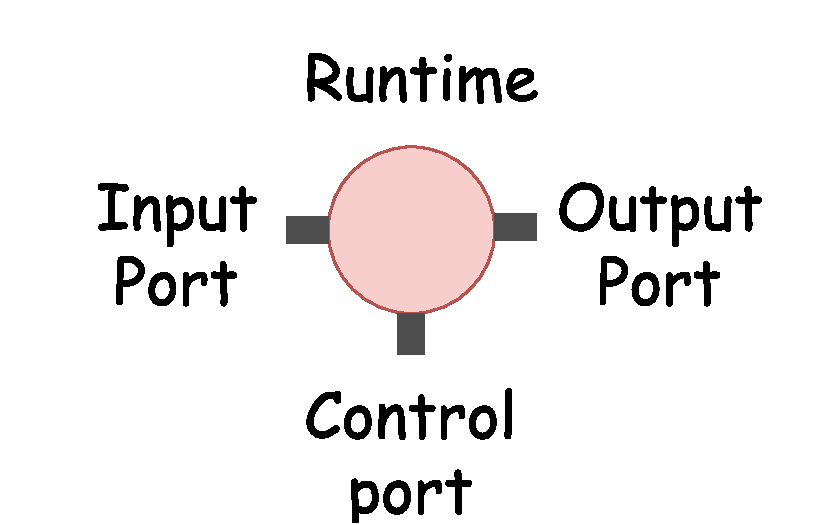
\includegraphics[width=\columnwidth]{figure/nfactor-runtime-with-port.pdf}
   \caption{A runtime with three ports.}\label{fig:runtime-with-port}
  \end{subfigure}\hfill
  \begin{subfigure}[t]{0.69\linewidth}
 \centering
   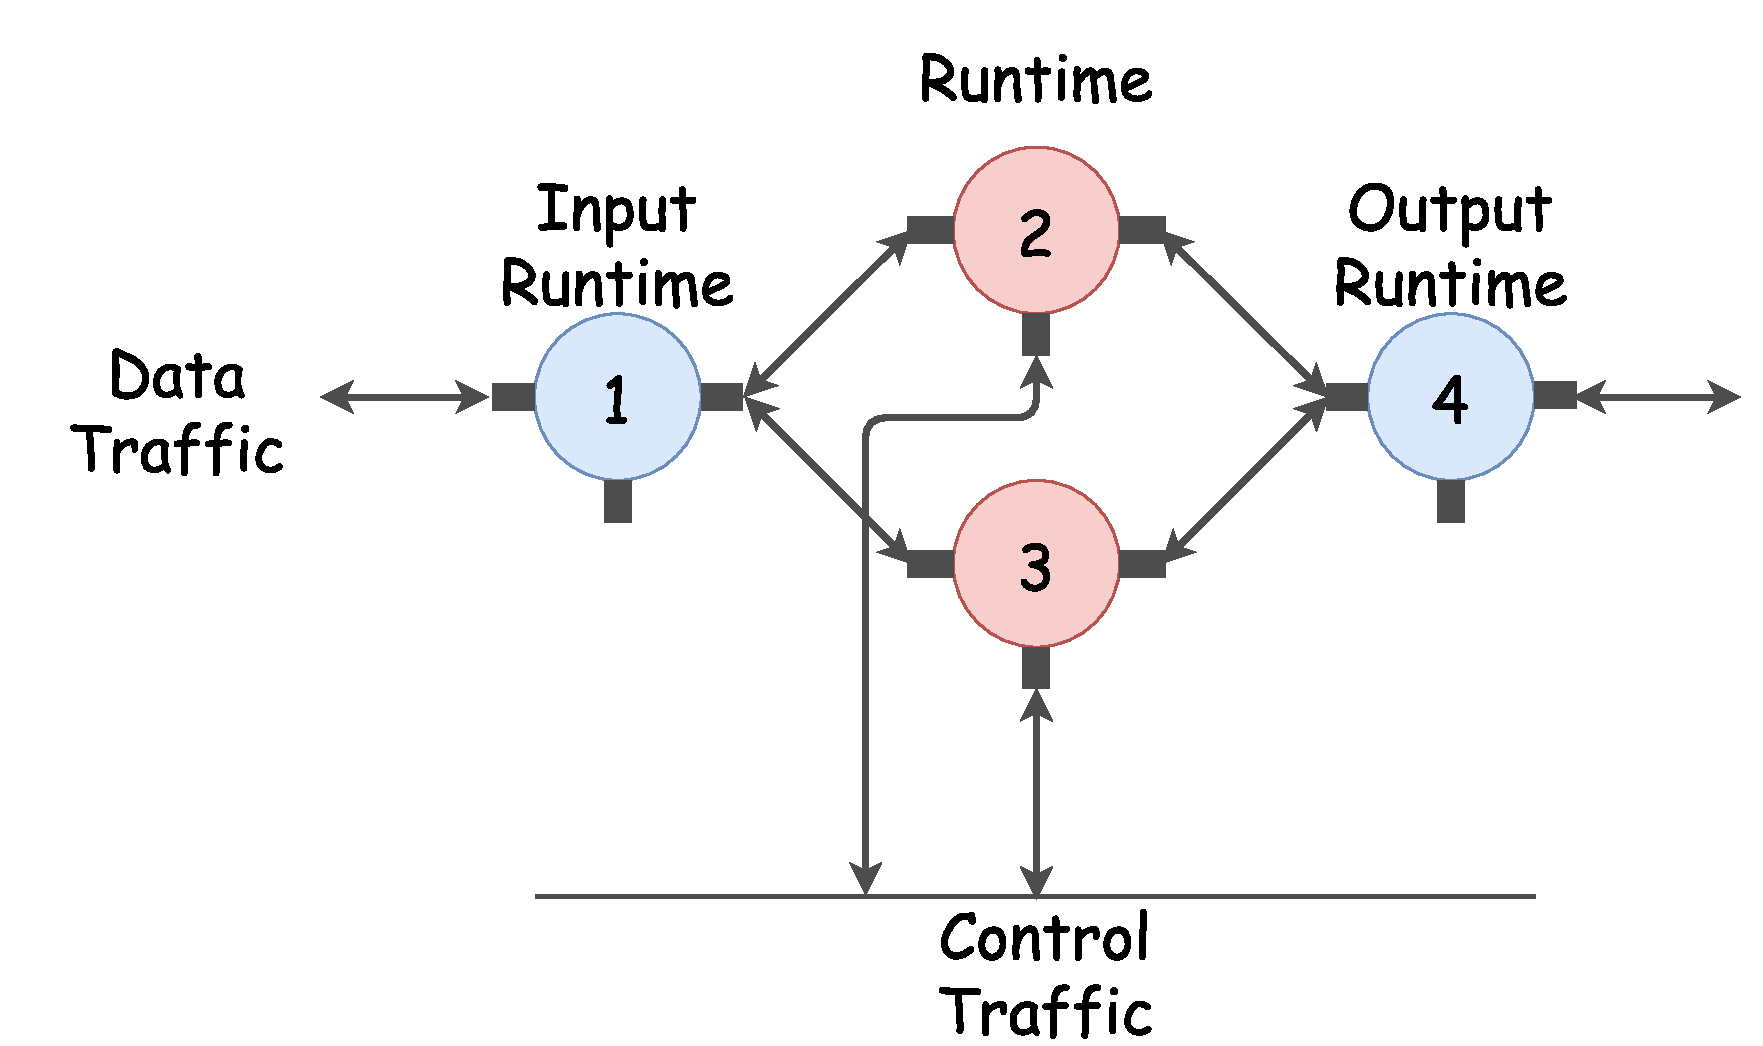
\includegraphics[width=\columnwidth]{figure/nfactor-runtime-connection.pdf}
   \caption{A minimal runtime connection.}\label{fig:runtime-with-io-runtime} \end{subfigure}\hfill
   \begin{subfigure}[t]{0.99\linewidth}
  \centering
    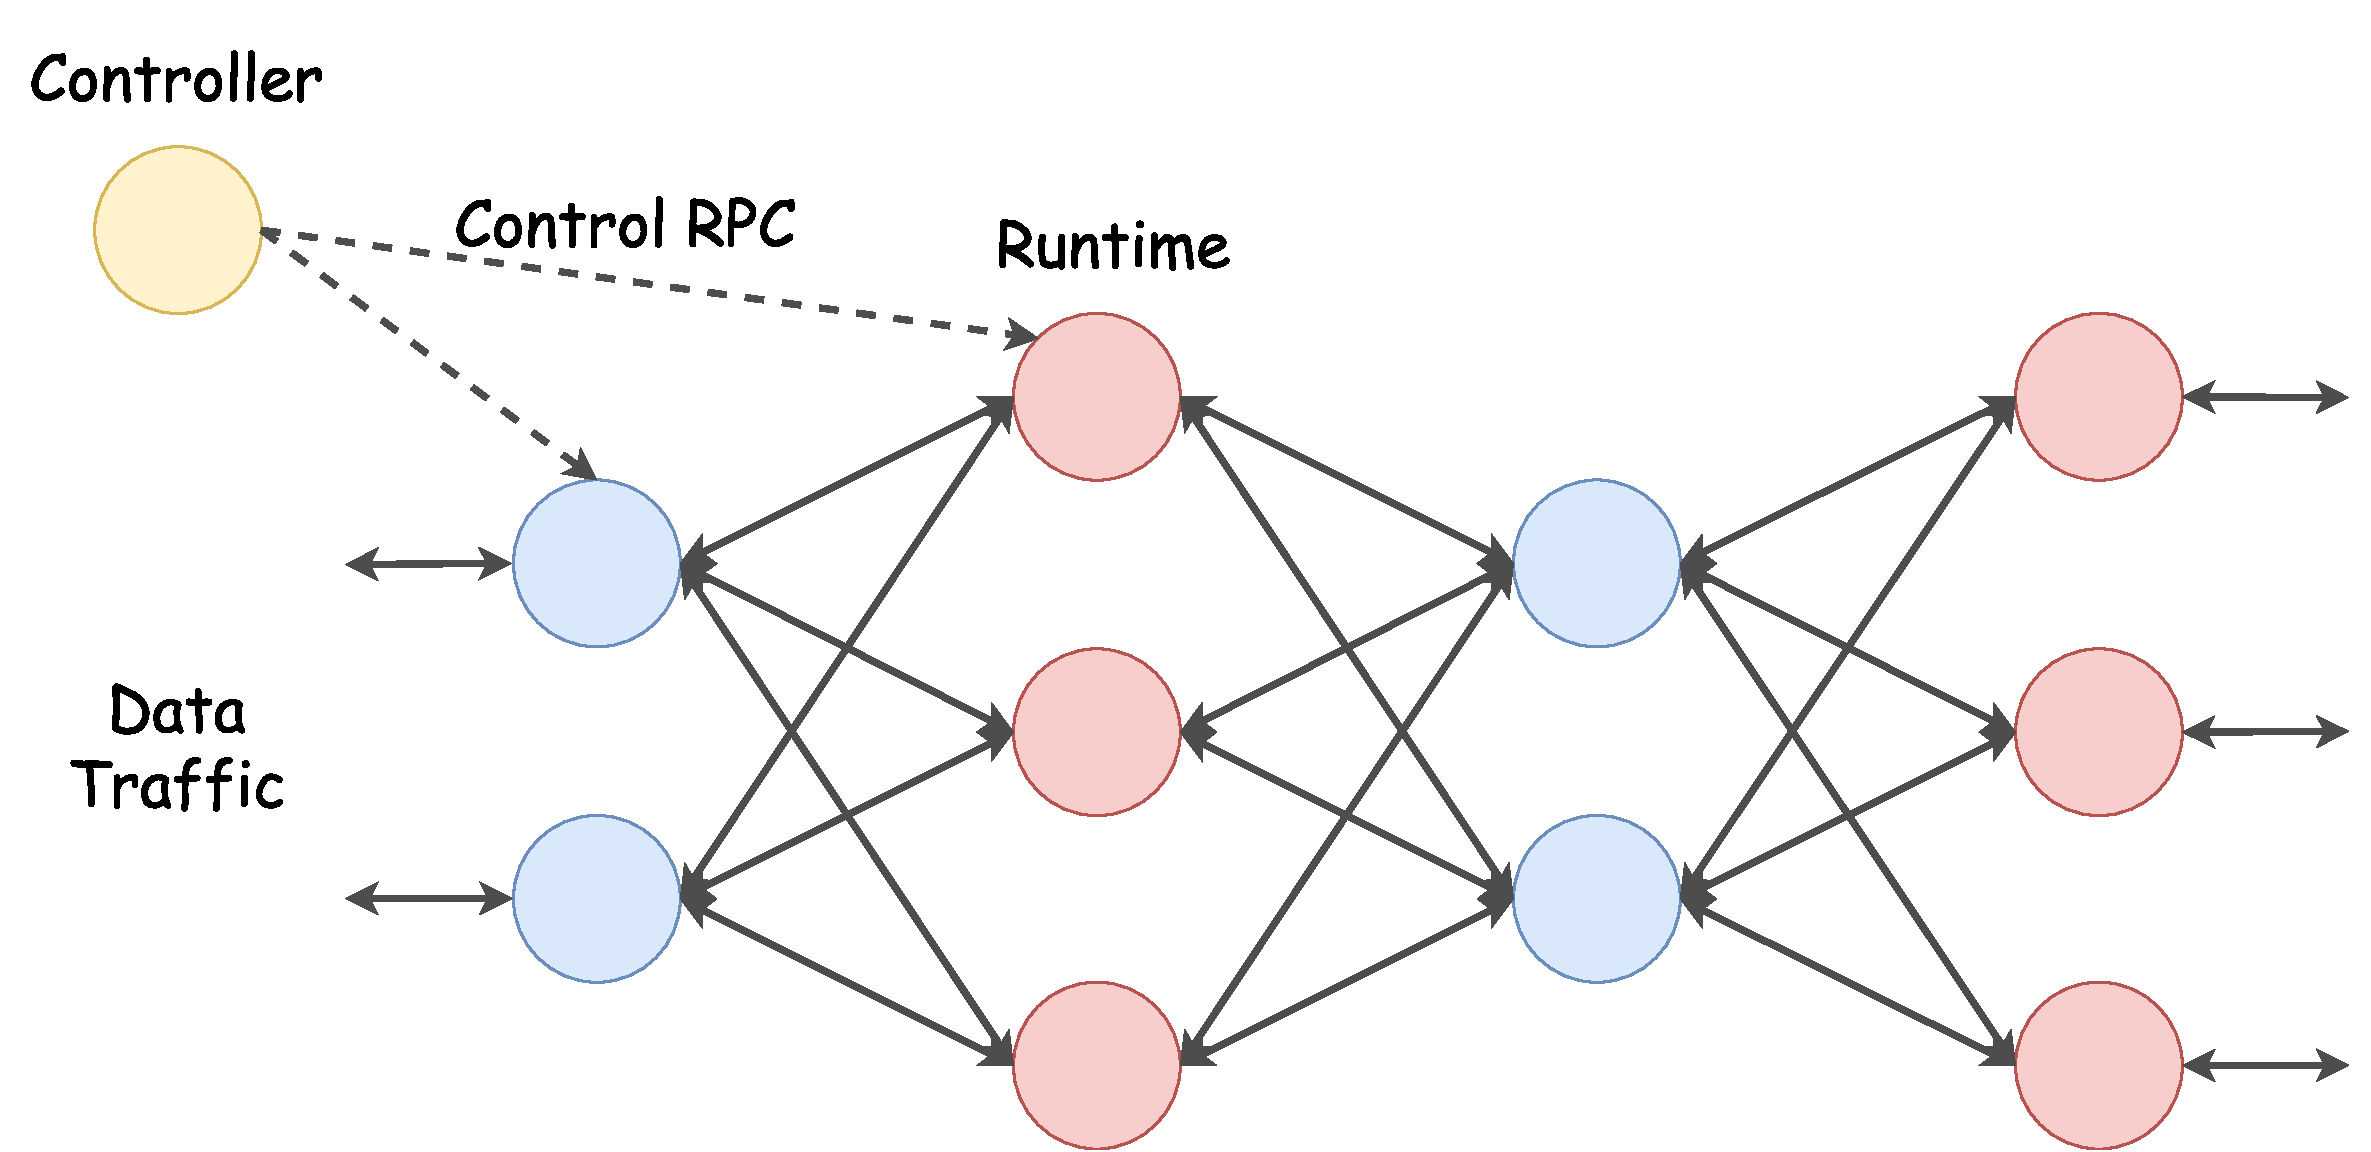
\includegraphics[width=\columnwidth]{figure/nfactor-cluster.pdf}
    \caption{A NFActor runtime cluster consists of multiple lay, controlled by a controller.}\label{fig:runtime-cluster} \end{subfigure}
 \caption{The flow migration performance of \nfactor}
\label{fig:runtime}
\end{figure}

%图1c展示了运行时cluster的基本结构。运行时cluster是由若干层运行时连接而成,并由一个轻量级的控制器利用RPC进行管理。
Figure \ref{fig:runtime-cluster} gives an example of a running NFActor cluster. The NFActor cluster consists of multiple runtimes controlled by a light-weight controller through RPC.

%图1a给出了一个runtime的基本结构。一个runtime包含三个端口。输入端口和输出端口用来接收和传递数据层的数据包。控制端口专门用来传递flow actor执行流管理任务时所生成的远程消息。输入输出端口也可以用来传递远程消息,我们在后面的章节中给出详细的解释。
Figure \ref{fig:runtime-with-port} shows the basic struture of a runtime. A runtime consists of three ports. The input and output ports are used to receive and send dataplane packets. The control port is only used to transmit remote messages when flow actor executes flow management tasks. Both input and output ports could also be used to transmit remote messages, this is further illustrated in later chapters.

%一个运行时系统自己并不能执行负载均衡以及流管理任务,它需要和其他的运行时系统进行连接才能完成这些功能。每一个运行时系统的三个端口都可以和其他多个运行是系统进行连接。图1b给出了一个能实现各种流管理功能的最小连接图。在图1b中,2号运行时系统的输入端口和输出端口分别与1号运行时系统的输出端口和4号运行时系统的输入端口相连,因此对于2号运行时系统而言,1号运行时系统时它的input runtime, 4号运行时系统时它的output runtime.同理,对于1号运行时系统而言,2号运行时系统时它的output runtime. 在NFActor framework中,运行时系统可以将自己的输出流量均匀分布在所有的输出运行时系统中。因此我们可以看到 dataplane traffic可以从图1b连接的一端进入并从另一端输出。

A runtime system could not execute any load-balacning and flow management tasks by itself. It needs to be connected with other runtimes and collaborate with those runtimes. The three ports of a single runtime system could be connected to multiple runtimes. Figure \ref{fig:runtime-with-io-runtime} gives a minimal runtime connection that is able to achieve load-balancing and flow management tasks. In figure \ref{fig:runtime-with-io-runtime}, the input and output ports of runtime 2 and 3 are connected with the output port of runtime 1 and input port of runtime 4. From the perspective of runtime 2, runtime 1 is its input runtime and runtime 4 is its output runtime. Similarly, runtime 2 is the output runtime of runtime 1. In NFActor framework, a runtime could balance its workload among all of its output runtimes. This is why the dataplane traffic could enter from one end of the connection in figure \ref{fig:runtime-with-io-runtime} and exit from the other end.

%对与2号和3号运行时系统而言,他们具有相同的input runtime和output runtime。我们将这一类运行时系统归纳入通一个layer。同一个layer的运行时系统的控制端口会被相互连接起来。同时,同一个layer的运行时系统之间可以实现快速高效的流迁移和容错。

From the perspective of runtime 2 and 3, they share the same input runtimes and output runtimes. These runtimes are classified into the same layer. The control ports of runtimes under the same layer are directly connected, so that flows could be quickly migrated and replicated among runtimes under the same layer.

%如图2所示,我们可以构建一个由multipile layers of runtime 所组成的nfactor cluster。这个cluster由一个轻量级的controller进行控制。controller可以检测每一个runtime的workload以实现动态扩展。同时,controller可以通过rpc来发起流管理任务的执行。

As shown in figure \ref{fig:runtime-cluster}, we can construct a NFActor cluster by creating multiple layers of runtimes. This runtime cluster could be controlled by a controller, which monitors the workload on each runtime for dynamic scaling. This controller could also initiate flow management tasks by sending RPC requests to selected runtimes. 

\begin{figure}
		\centering
		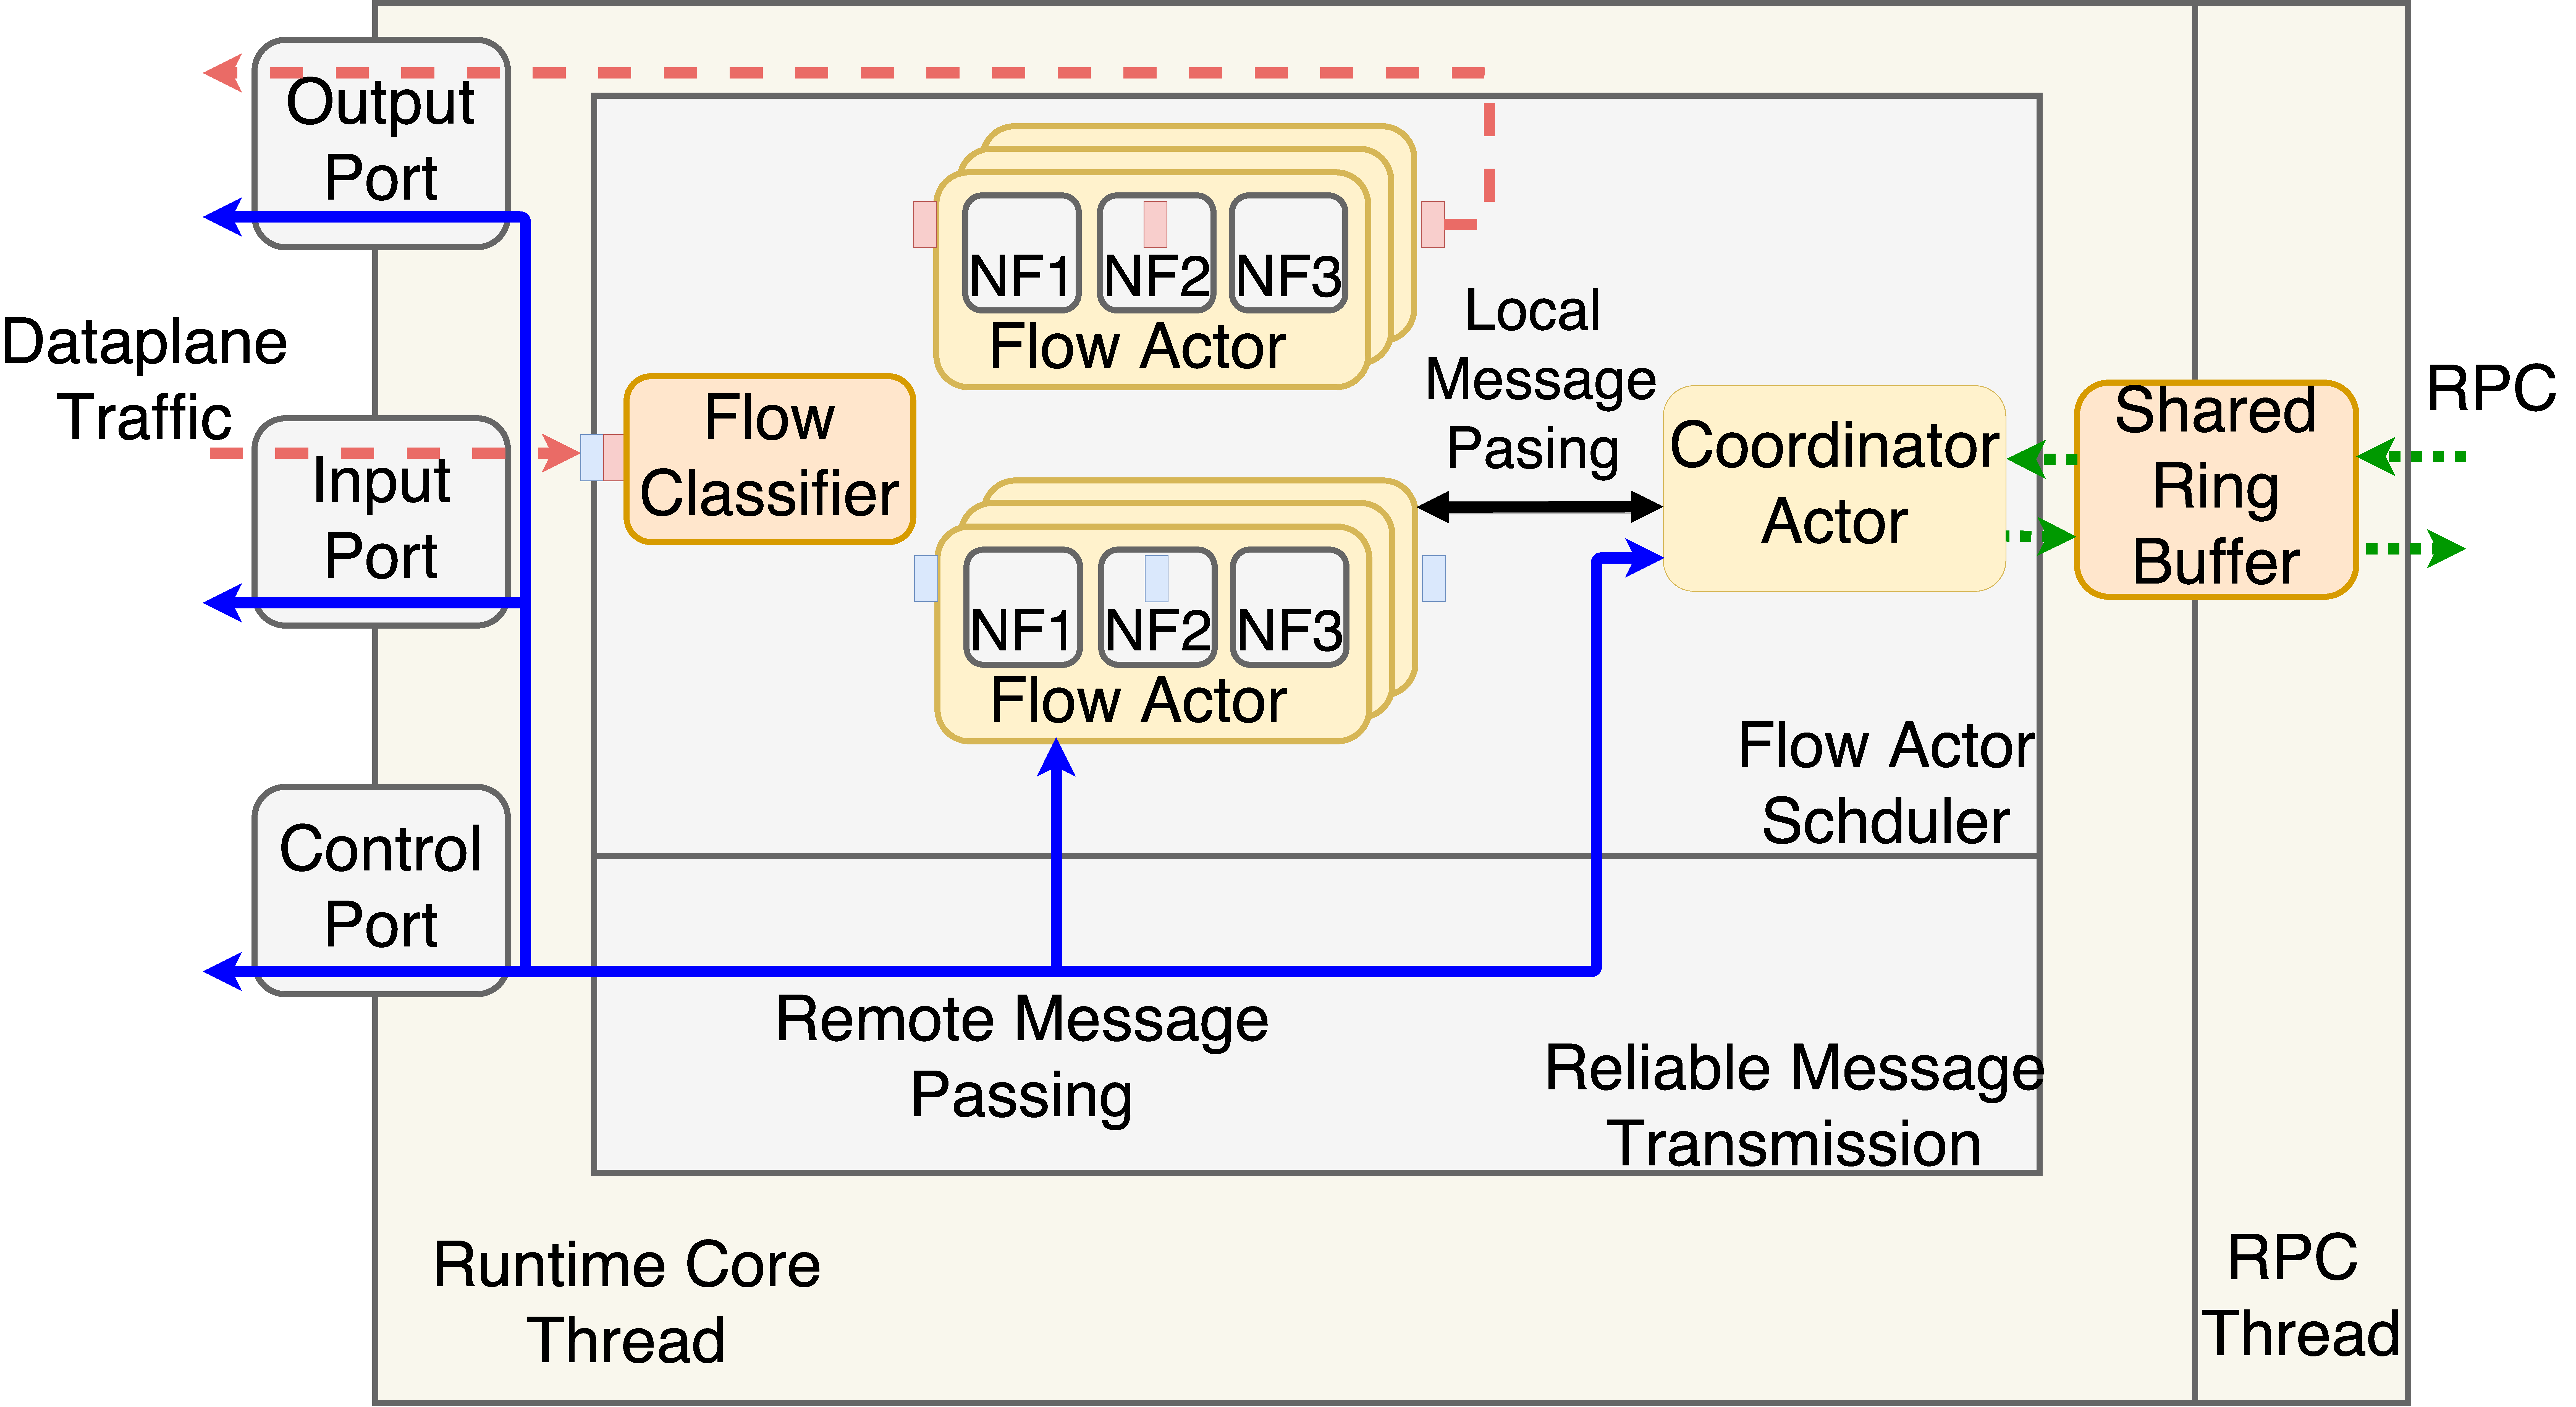
\includegraphics[width=\columnwidth]{figure/nfactor-runtime-arch.pdf}

		\caption{The internal architecture of a NFActor runtime system. }
\label{fig:runtime-arch}
\end{figure}

%\section{Resilience}

In this section, we present the fault tolerance mechanism and flow migration protocol used by NFActor framework. Before going into the details, we first compare the difference between 

\subsection{Fault Tolerance}
\label{sec:ft}

In this section, we introduce the fault tolerance mechanisms for our NFActor
framework, including the controller, the virtual switch, and the runtimes. 
Depending on the nature of these three components, we carefully design 
lightweight fault-tolerance mechanisms for them so that these mechanisms be 
robust and have little performance impact in normal case.

\subsubsection{Replicating Controller}

Since the controller is a singled-threaded server that stores the states of 
the NFActor runtime, we persistently log these states and replicate them. The 
controller only needs to log the state of each NFActor runtime in 
the cluster view list. Whenever the controller needs to modify the state of a 
runtime, it logs the intended operation, modifies the state and logs a success 
mark for the intended operation.

The liveness of the controller is monitored by a guard process and the 
controller is restarted immediately in case of failure. On a reboot, the 
controller reconstructs the state in the cluster view list by replaying log. 
Each runtime in the cluster monitors the connection status with the controller 
and reconnects to the controller in case of a connection failure.

\subsubsection{Replicating Virtual Switch}

The most important state of the virtual switch process is its switching hash 
table in memory. In order to replicate the virtual switch, we constantly 
check-point the container memory image of the virtual switch using CRIU 
\cite{criu}, a popular tool for checkpoint/restore Linux processes. One main 
technical challenge is that CRIU has to stop a process before checkpointing it, 
which may hurt the availability of the virtual switch.

We tackle this challenge by letting the virtual switch call a 
fork() periodically (by default, one minute), and then we use CRIU to checkpoint 
the child process. Therefore, the virtual switch can proceed without affecting 
NFActor performance.

% Since the
% check-pointing needs to halt the execution of the whole virtual switch, it can
% not be frequently performed. In our implementation, we create a check-point for
% every second. However, this means that some states in the switching hash table
% might be lost and the flow connection related with these states may be forced to
% terminate. We argue that this is an acceptable implementation trade-off as flows
% could do a reconnection to complete unfinished tasks. If strong consistency is
% required, the virtual switch could use the replication strategy of
% FTMB\cite{sherry2015rollback}, we leave this to the future work.

\subsubsection{Replicating Runtime}

\begin{figure}
	\begin{subfigure}[b]{0.45\columnwidth}
		\centering
		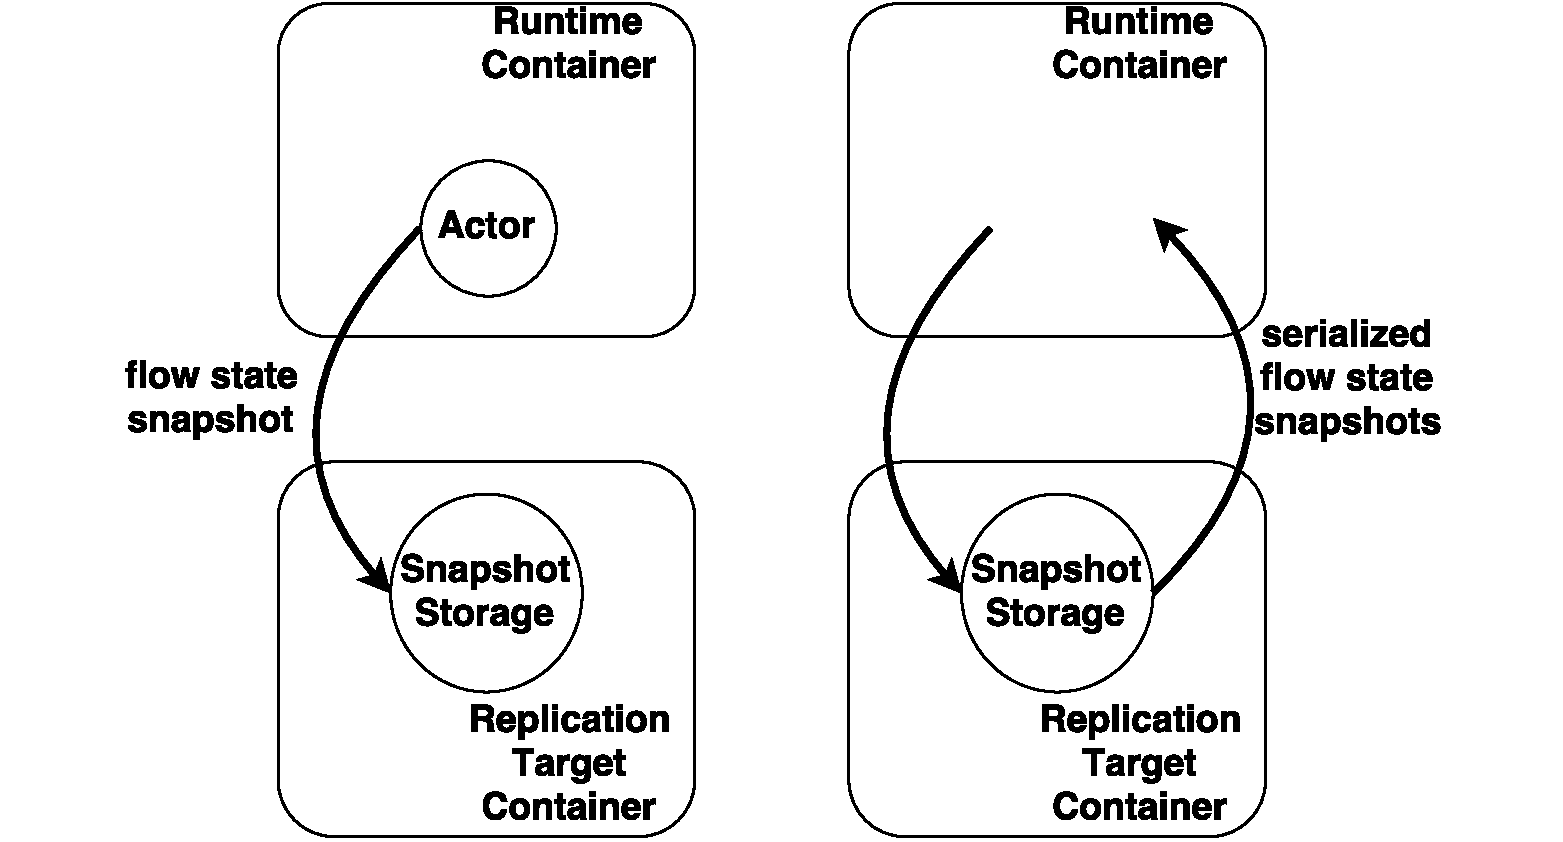
\includegraphics[width=\columnwidth]{figure/NFActor-Runtime-Replicate.pdf}
		\caption{Actor replicates its flow state to another
		runtime.}\label{fig:replicate} \end{subfigure}\hfill
	\begin{subfigure}[b]{0.45\columnwidth}
		\centering
		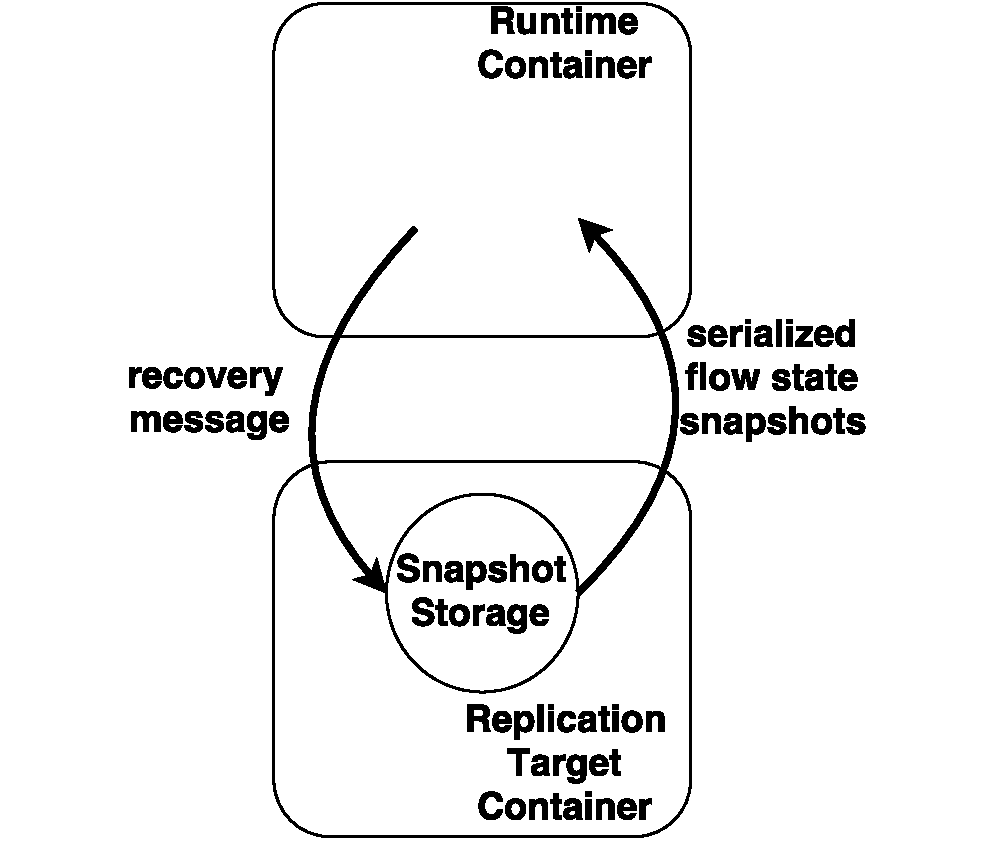
\includegraphics[width=\columnwidth]{figure/NFActor-Runtime-Recover.pdf}
		\caption{A failed runtime is restarted.}\label{fig:recover}
	\end{subfigure}%
\caption{Replication strategy for NFActor runtime.}
\end{figure}

To perform lightweight NFActor runtime replication, we leverage the actor 
abstraction and state separation to create a lightweight flow state replication 
strategy. In NFActor runtime, important flow states associated with a flow is 
owned by a unique actor. NFActor runtime can replicate each actor 
independently without incurring the overhead of check-pointing the entire 
container images \cite{sherry2015rollback, rajagopalan2013pico}.

This primary-backup replication manner can tolerate one actor failure at 
runtime, and we think this fault-tolerance guarantee is sufficient because the 
chance two actor machines failing at the same time is extremely rare.

\textbf{Find A Replication Target}: When the actor is created, it selects a
\textit{running} state runtime with the smallest workload as its replication
target. Then the actor negotiates with the replication target about whether the
replication target can accept this actor's replica. In case that replication
target refuses to store the actor's replica, the actor tries to select
another replication target. 

\textbf{Flow State Replication (figure \ref{fig:replicate})}: After determining
the replication target, the actor performs flow state replication. Before the input packet is processed on
the service chain, the actor saves a copy of the input packet. After the packet
finishes being processed on the service chain, the actor sends the local runtime
ID, flow identifier, original input packet and the processed packet to the
replication target. For every fixed number of packets that the actor has processed, the actor create a
snapshot of all the flow states and send the snapshot to the replication target as well.

When the replication target receives a new replication message, it saves the
message content in the RAM. If received message includes a new state snapshot,
replication target wipes out all previously saved content associated with the flow and save the new
state snapshot as well. Then the replication target sends the processed
packet out from its output port to the virtual switch. The flow state
replication procedure ensures the same output commit property as indicated in
\cite{sherry2015rollback}.

\textbf{Recover Failed Runtime (figure \ref{fig:recover})}: If a NFActor runtime
fails, it's failure will be detected by the controller after a timeout. Then the failed NFActor runtime will be restarted
with the same runtime ID. The restarted NFActor then starts recovery process. It
sends to all the other NFActor runtimes in the cluster a recover message, which
contain its NFActor runtime id. Other NFActor runtimes respond to the recover
message by sending all the replicas with the same runtime ID back to the
restarted NFActor runtime. The restart NFActor runtime then use these replicas
to reconstruct its state before failure. When the NFActor runtime finishes
recovery, it sends a {\tt join} message back to the controller to re-join the
cluster. 

% \textbf{Discussion}: The runtime replication strategy can tolerate at most one
% failed runtime. If multiple runtimes fail concurrently, then the replicas will
% be lost and the states of some flows will never be correctly recovered.
% Multi-machine replication algorithm such as PAXOS \cite{chandra2007paxos} could
% be used to replicate the flow state to multiple backups. However, PAXOS may not
% be efficient enough to handle the replication of a large number of packets. We
% leave exploring multi-backup to our future work. 

%%%%%%%%%%%%%%%%%%%%%%%%%%%The following is flow migration%%%%%%%%%%%%%%%%%%%%%%%%%

\subsection{Distributed Flow Migration}
\label{sec:fm}

In this section, we present the distributed flow migration method of NFActor
framework. There are some problems with existing flow migration
framework \cite{gember2015opennf, rajagopalan2013split}. First they all use a
centralized controlelr to monitor the entire flow migration
process. This is not scalable. The second problem is that the flow migration
protocol is too complicated to implement. Patch code needs to be added to the
core processing logic of the NFs. The flow migration protocol needs to exchange
multiple messages among controller, switches and NF instances. This increases
the possibility of serious software bugs. The final problem is that the NF can
not start the flow migration process by itself. It must be started from the
controller. This stops the NFs from making timely responses to overload signal.

All the above mentioned problems could be solved using NFActor framework. In
NFActor framework, the NF packet processing is carried out within the
execution context of the actor. This additional layer of monitoring gives
NFActor power to start flow migration from the NFActor runtime. On the other
hand, the API design forces a clean separation between flow state and NF
processing logic, making extracting and serializing flow state an easy task.
NFActor framework also has a built-in message-passing functionality that
makes flow migration simpler. In this section, we elaborate in detail how flow
migration works in NFActor framework.

\subsubsection{Distributed Flow Migration Protocol}

\begin{figure*}[!t]
	\begin{subfigure}[t]{0.23\linewidth}
		\centering
		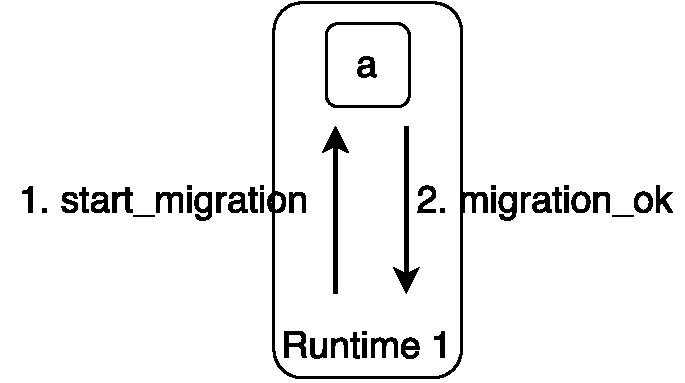
\includegraphics[width=\columnwidth]{figure/NFActor-Flow-Migration-Init.pdf}
		\caption{Initiate flow migration.}\label{fig:init} 
	\end{subfigure}\hfill
	\begin{subfigure}[t]{0.23\linewidth}
		\centering
		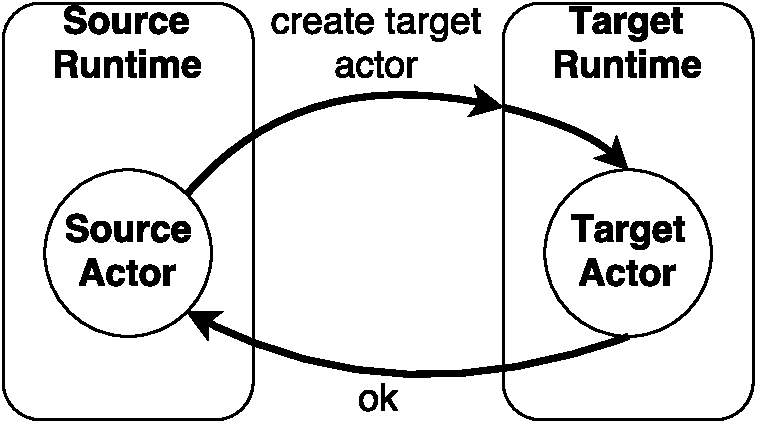
\includegraphics[width=\columnwidth]{figure/NFActor-Flow-Migration-First.pdf}
		\caption{Create target actor.}\label{fig:first} \end{subfigure}\hfill
	\begin{subfigure}[t]{0.23\linewidth}
		\centering
		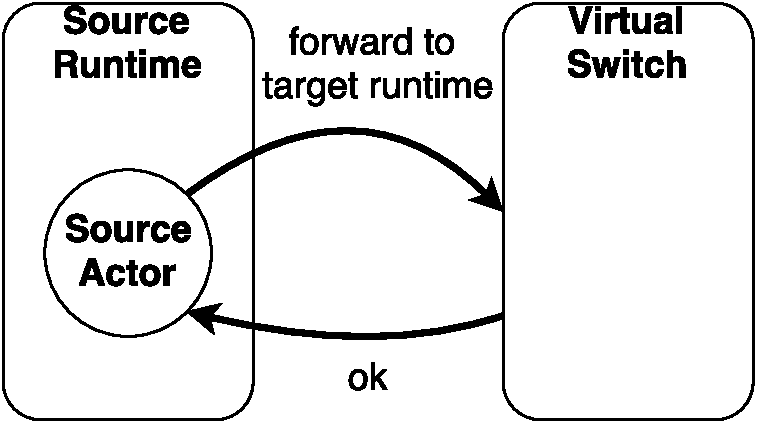
\includegraphics[width=\columnwidth]{figure/NFActor-Flow-Migration-Second.pdf}
		\caption{Contact virtual switch.}\label{fig:second}
	 \end{subfigure}\hfill
	 \begin{subfigure}[t]{0.23\linewidth}
		\centering
		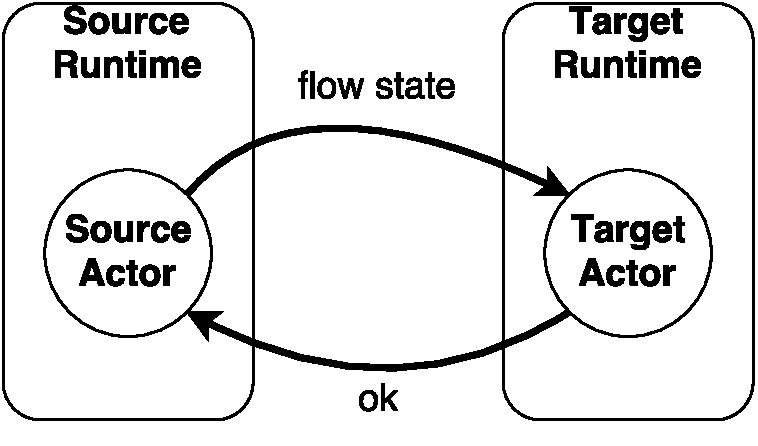
\includegraphics[width=\columnwidth]{figure/NFActor-Flow-Migration-Third.pdf}
		\caption{Migrate flow state.}\label{fig:third}
	 \end{subfigure}
\caption{Distributed Flow Migration Protocol of NFActor Framework}
\label{fig:migration}
\end{figure*}

The distributed flow migration protocol is shown in figure \ref{fig:migration}.
It consists of passing 4 request-response. We first show successful
request-response in figure \ref{fig:migration} and then supplement possible
failure cases.

\textbf{Initiate Flow Migration}: As shown in figure \ref{fig:init}, the flow
migration in NFActor is initiatied by sending a {\tt start\_migration} message
from the NFActor runtime 1 to an actor \textit{a} on this runtime. The {\tt
start\_migration} message contains a ID of a target runtime. Runtime 1 acquires
this ID by querying the view service. Once actor \textit{a} receives this
message, it starts the migration process by itself, without involving a centralized controller.

Runtime 1 is promised to receive a response from actor \textit{a}. A {\tt
migration\_ok} message sent from actor \textit{a} indicates that the migration
is successfully finished. The flow being migrated has
resumed its execution on the target runtime. Actor \textit{a} has quit
execution and released all its resources. The migration can of course fail due
to many reasons. In that case, actor \textit{a} will respond a {\tt
migration\_fail} message back to runtime 1 and continue to process flow packets
on runtime 1.

\textbf{Create Target Actor:} Actor \textit{a} then sends a {\tt create\_target\_actor} request message to the
target runtime 2, expecting a response. This message also contains the flow
identifier of actor \textit{a}. Target runtime 2 target runtime 2 creates a target
actor \textit{b}, registers target actor \textit{b} using the flow identifer
contained in the {\tt start\_migration} message and delegates the migration
process to target actor \textit{b}. Target actor \textit{b} then responds a {\tt
ok} message to actor \textit{a}.

\textbf{Contact Virtual Switch:} Actor \textit{a} sends a {\tt
forward\_to\_target\_runtime} request message to the virtual switch. This
message contains the flow identifier and the ID of the target runtime 2. After
virtual switch has received the request message, the virtual switch first
updates its switching hash table by changing the value associated with the flow identifier
to the ID of target runtime 2. Then the virtual switch creates a data-plane
packet with the same flow identifier contained in the message and fills the
payload with a global unique magic-number. Then the virtual switch sends this
data-plane packet back to runtime 1.

When actor \textit{a} receives the data-plane packet with the magic number, it
knows that the no more flow packets will be forwarded to itself. Then actor
\textit{a} can safely migrate its flow state to the target actor \textit{b}. The
use of the data-plane packet instead of control message ensures lossless flow
migration \cite{gember2015opennf}. In case that actor \textit{a} fails to
receive data-plane response packet after a timeout, actor \textit{a} will
re-send {\tt forward\_to\_target\_runtime} to the virtual switch.

After virtual switch updates its switching hash table, target actor \textit{b}
starts to receive flow packets. Target actor \textit{b} only buffers these
packets and waits until flow state migration complete before processing them.

\textbf{Migrate Flow State:} Actor \textit{a} sends a {\tt migrate\_flow\_state}
request message, along with the serialized flow states of actor \textit{a}, to
target actor \textit{b}. After receving the request message, target actor
\textit{b} first responds a {\tt ok} message back to actor \textit{a}.
Then it drains all the buffered packets and resumes normal flow packet
processing. 

Actor \textit{a} on the other hand, waits until it receives {\tt ok} message
from target actor \textit{b}. Then it responds a {\tt migration\_ok} message
back to runtime 1, destroies all the of its resources and quits.

\subsubsection{Failure Handling}
 
The flow migration protocol in figure \ref{fig:first} to \ref{fig:third} may
generate different kinds of failures. This causes actor \textit{a} in figure
\ref{fig:init} to responds a {\tt migration\_fail} message back to runtime 1. In
this section, we analyze possible failures and how to handle these failures.
Flow migration protocol relies on failure recovery to handle some serious
failures. For the flow migration process, the target actor does not maintain a
replica. In the meantime, the actor being migrated does not log that it is being
migrated. This means that if the runtime involved in the migration fails, the
migration is implicitly stopped.

\textbf{Target runtime is overloaded.} In figure \ref{fig:first},
when target runtime 2 receives {\tt create\_target\_actor} message, it first
checks whether it is overloaded before creating target actor \textit{b}.
This is because runtime 1 uses the view service to determine target runtime and
the view service is not an always-up-to-date service. Target runtime 1 may
experience overload and it can not accept new migrated actors. In that case,
target runtime 2 respond a {\tt fail} response back to actor \textit{a}, causing
actor \textit{a} to stop the migration.

\textbf{Messages are lost in the network.} In figure \ref{fig:first}, if either
the {\tt create\_target\_actor} message or the response message is lost, actor
\textit{a} stops migration. This also causes a timeout to be triggered on target
actor \textit{b} and stops \textit{b}. Figure \ref{fig:second} and
\ref{fig:third} involve changing packet forwading path and migrating flow state.
The migration can not be simply stopped due to message loss. In figure
\ref{fig:second}, actor \textit{a} just keeps re-sending the request message
until it receives a definitive response. In figure \ref{fig:third}, actor
\textit{a} keep retrying for a fixed number of times. Then it performs a live
recovery.

\textbf{Runtime fails.} In figure \ref{fig:first}, the failure of either runtime
simply halts the migration process. In figure \ref{fig:second} and
\ref{fig:third}, actor \textit{a} and target actor \textit{b} monitor each
other. The failure of runtime 1 causes target actor \textit{b} not to receive
{\tt migrate\_flow\_state} message. Actor \textit{b} requests the virtual switch
to forward to runtime 1. The failure of target runtime 2 causes actor \textit{a}
to perform a live recovery. 

\textbf{Buffer Overloads.} After virtual switch updates its switching hash
table, target actor \textit{b} starts to buffer the packets. We set a maximum
capacity for the buffer. If the buffer is full when receiving {\tt
migrate\_flow\_state} message, target actor \textit{b} responds a {\tt fail}
message to actor \textit{a}, causing \textit{a} to perform a live recovery.

\textbf{Virtual Switch Fails.} After virtual switch is restarted, it may lost
some states in the switching hash table. The flow being migrated may be forced
to terminate due to inconsistent state.










\section{Implementation}
\label{sec:implementation}

%Discuss the implementation details here. 

%\chuan{give thresholds used to detect overload and idling of runtimes; give the fixed number for ``For every fixed number of packets that the actor has processed"}

The implementation of the core functionalities of NFActor framework consists of 9921 lines of C/C++ code, excluding the implementation of 3 customized NF modules and miscellaneous helper codes. In NFActor, each runtime is containerized using Docker. The data plane of NFActor is inter-connected using BESS \cite{Han:EECS-2015-155}, which is a virtual switch for implementing high performance NFV system. The control plane of NFActor is inter-connected using OpenVSwitch \cite{pfaff2015design}. The actor runtime is implemented using libcaf \cite{caf}, which is a C++ actor programming framework. 

The internal implementation of NFActor runtime is separated into 2 parts, which are a packet polling thread and several actor worker threads. The packet polling thread polls the input queue created by the BESS for packets and fetches the packets directly from the huge page memory area \cite{dpdk}. Then the packet polling loop sends the packet to a actor as an actor message. All the actors are scheduled to run on the worker threads. When the actor gets it's schedule to run, it processes as many received messages as possible. When the actor finishes processing a packet, it sends the packet back to the packet polling loop through a lockless multi-producer queue. The packet polling loop in turn sends the packet to the outside world. 




\section{Evaluation}
\label{sec:experiments}

%Evaluate \nfactor system.

%\chuan{remember to show how many lines of code or other overhead needed for implementing NFV anew on the actor framework}

We evaluate \nfactor framework using a Dell R430 Linux server, containing 20 logical cores, 48GB memory and 2 Intel X710 10Gb NIC. In our evaluation, we run the controller process, helper deamon process, virtual switch container and runtime containers on the same server. 

To evaluate the performance of \nfactor, we implement 3 customized NF modules using the API provided by \nfactor~framework, the 3 NF modules are flow monitor, firewall and HTTP parser. The flow monitor updates an internal counter when it receives a packet. The firewall maintains several firewall rules and checks each received packet against the rule. If the packet matches the rule, a tag in the flow state is flipped and later packets are automatically dropped. The firewall also records the connection status of a flow in the flow state. For the HTTP parser, it parses the received packets for the HTTP request and responses. The requests, responses and the HTTP method are saved in the flow state. Throughout the evaluation, we use a service chain consisting of  ``flow monitor$\rightarrow$firewall$\rightarrow$http parser'' as the service chain. We generate evaluation traffic using the BESS's FlowGen module and we directly connect the FlowGen module to the external input port of the virtual switch.

%Table goes  here to explain the functionalities of the NF modules.

The rest of the section tries to answer the following questions. \textit{First, } what is the packet processing capacity of \nfactor~framework? (Sec. \ref{sec:ppc}) \textit{Second, } how well is \nfactor~scales, both in terms of the number of worker threads used by a runtime and the number of runtimes running inside the system? (Sec. \ref{sec:ppc}) \textit{Third, } how good is the flow migration performance of \nfactor~framework when compared with existing works like OpenNF? (Sec. \ref{sec:fmp}) \textit{Fourth, } what is the performance overhead of flow state replication and does the replication scale well? (Sec. \ref{sec:rp})

 \subsection{Packet Processing Capacity}
 \label{sec:ppc}
 
 \begin{figure}[!t]
	\begin{subfigure}[t]{0.49\linewidth}
		\centering
		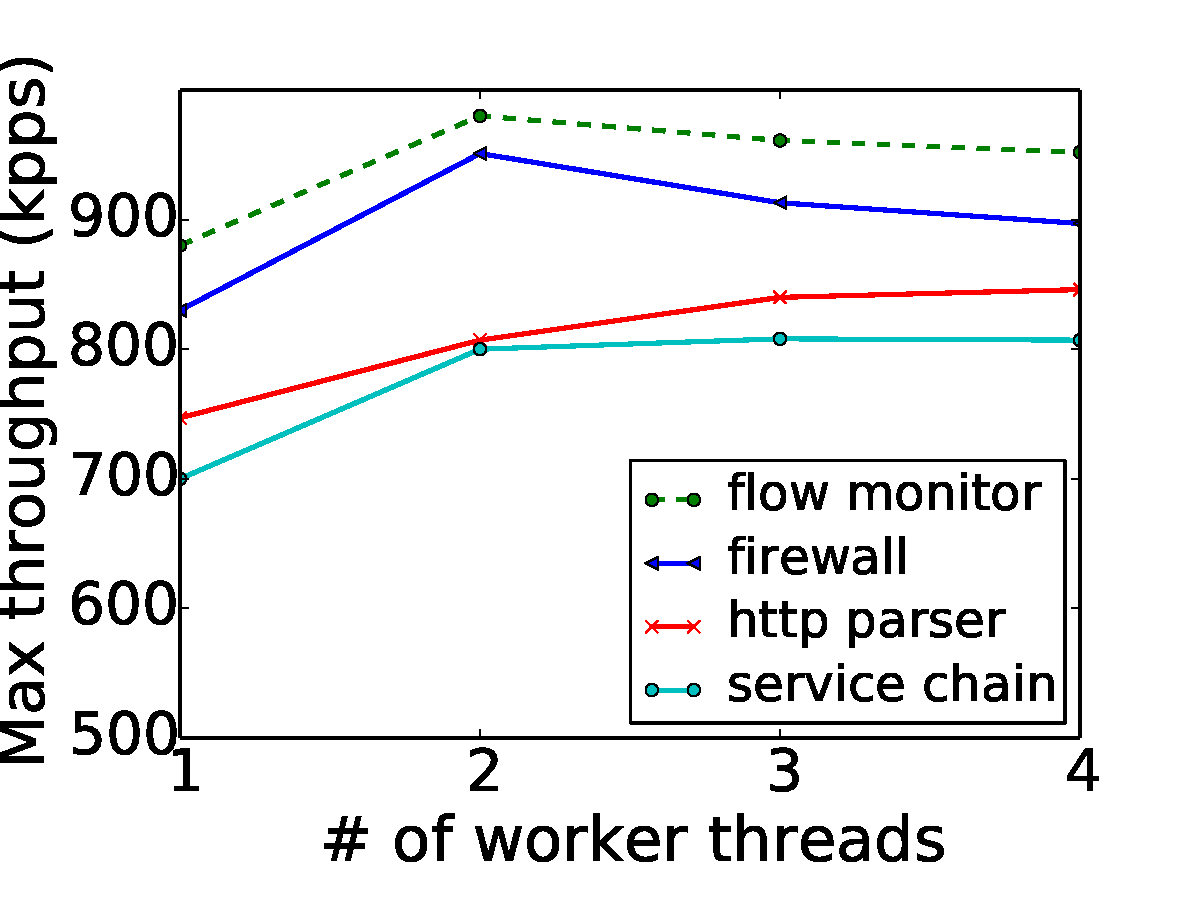
\includegraphics[width=\columnwidth]{figure/nf_throughput_evaluation.pdf}
		\caption{Packet processing capacity of a single \nfactor~runtime system running with different number of worker threads.}\label{fig:normal-performance} \end{subfigure}\hfill
	 \begin{subfigure}[t]{0.49\linewidth}
		\centering
		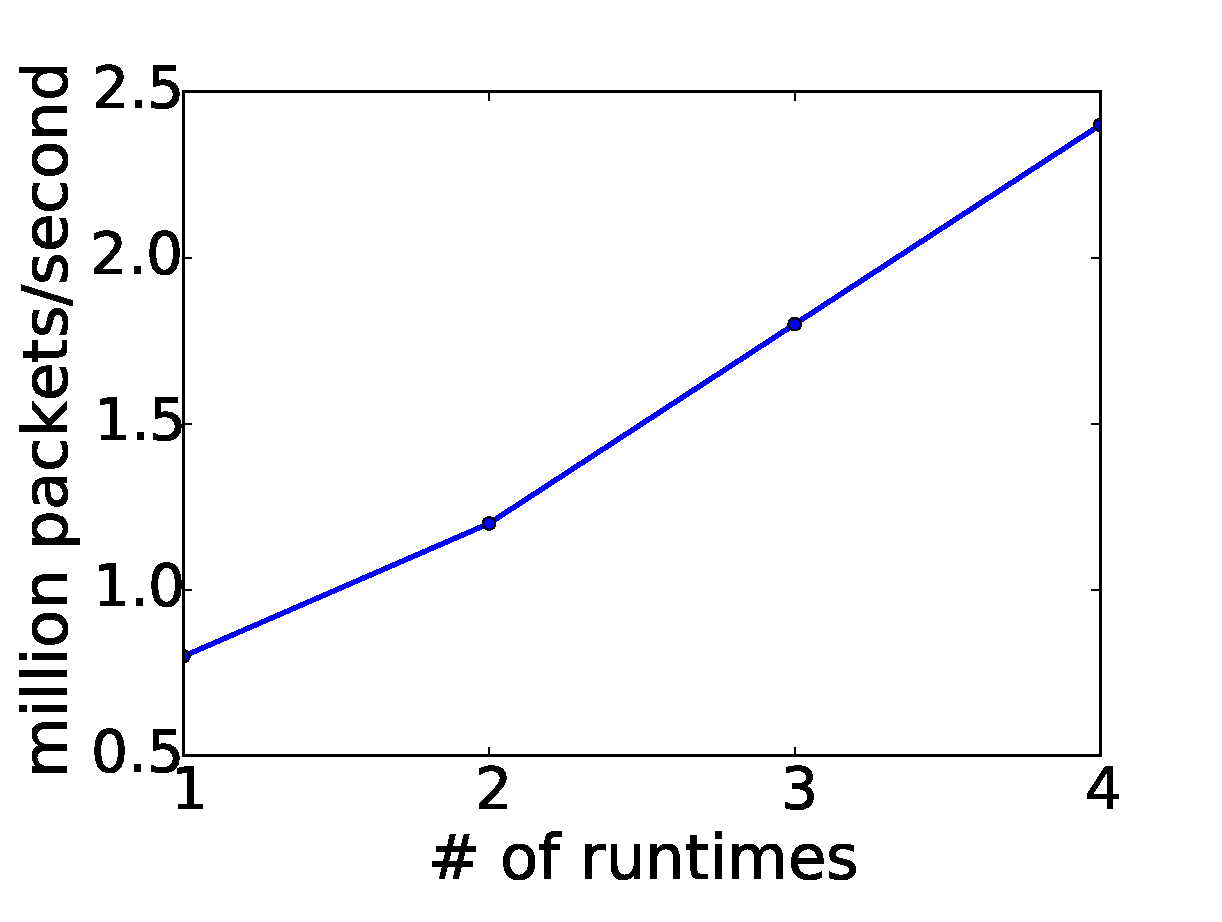
\includegraphics[width=\columnwidth]{figure/runtime_pktthroughput.pdf}
		\caption{Aggregate packet processing capacity of several \nfactor~runtimes.}\label{fig:scalability-performance}
	 \end{subfigure}
\caption{The performance and scalability of \nfactor~runtime, without enabling flow migration }
\label{fig:performance}
\end{figure}

Figure \ref{fig:performance} illustrates the normal case performance of running \nfactor~framework. Each flow in the generated traffic has a 10 pps (packet per second) per-flow packet rate. We vary the number of concurrently generated flows to produce varying input traffics. In this evaluation, we gradually increase the input packet rate to the \nfactor~cluster and find out the maximum packet rate that the \nfactor~cluster can support without dropping packets. In figure \ref{fig:normal-performance}, the performance of different NF modules and the service chain composed of the 3 NF modules are shown. Only one \nfactor~runtime is launched in the cluster. It is configured with different number of worker threads. In figure \ref{fig:scalability-performance}, we create different number of \nfactor~runtimes and configure each runtime with 2 worker threads. Then we test the performance using the entire service chain.

From figure \ref{fig:normal-performance}, we can learn that the packet throughput decreases when the length of the service chain is increased. Another important factor to notice is that the \nfactor~runtime does not scale linearly as  the number of worker threads increases. The primary reason is that inside a \nfactor~runtime, there is only one packet polling thread. As the number of input packets increases, the packet polling thread will eventually become the bottleneck of the system. However, \nfactor~runtime scales almost linearly as the total number of \nfactor~runtimes increases in the cluster. When the number of runtimes is increased to 4 in the system, the maximum packet throughput is increased to 2.4M pps, which confirms to the line speed requirement of NFV system. 

\subsection{Flow Migration Performance}
\label{sec:fmp}

 \begin{figure}[!t]
	\begin{subfigure}[t]{0.49\linewidth}
		\centering
		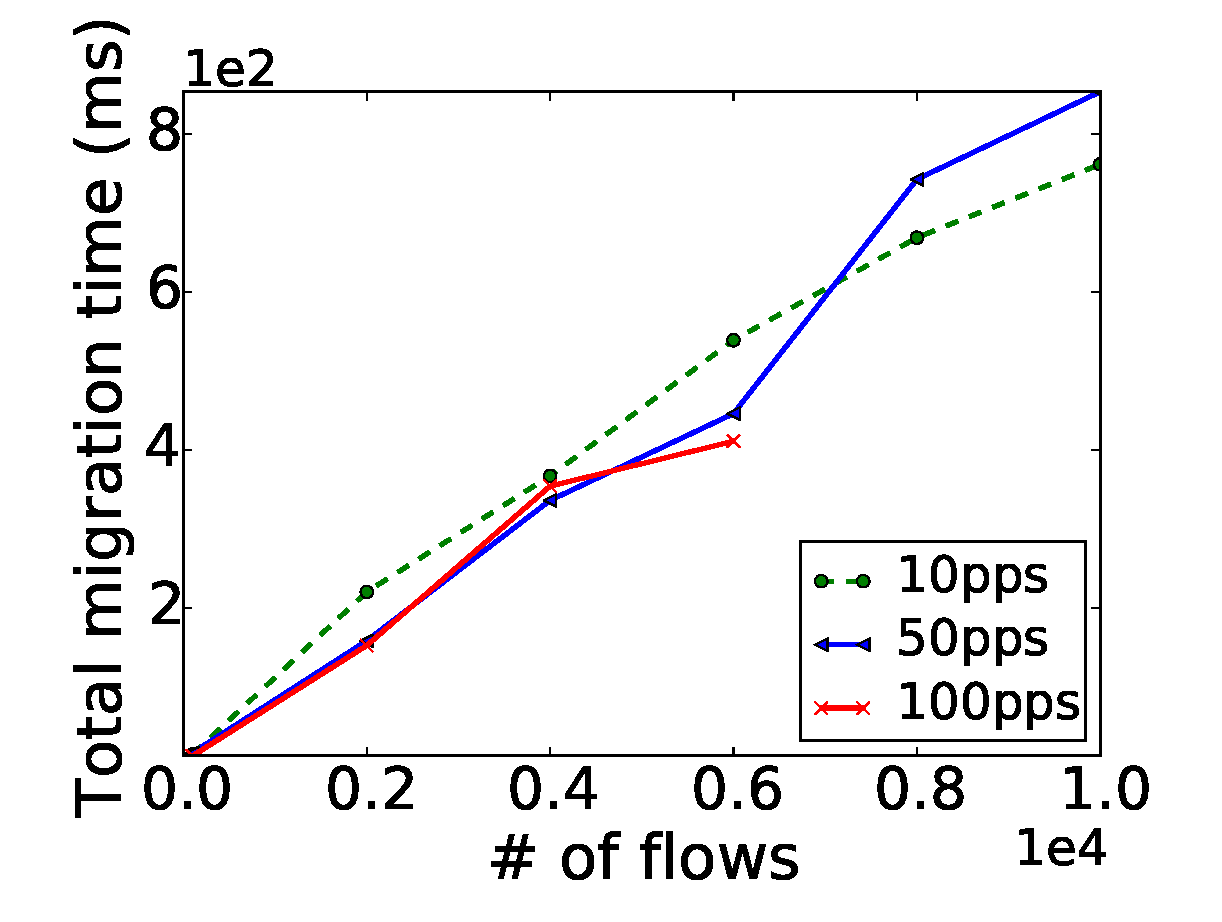
\includegraphics[width=\columnwidth]{figure/multi_flows_tot_migration_time.pdf}
		\caption{The total time to migrate different numbers of flows.}\label{fig:tot-mig} \end{subfigure}\hfill
	 \begin{subfigure}[t]{0.49\linewidth}
		\centering
		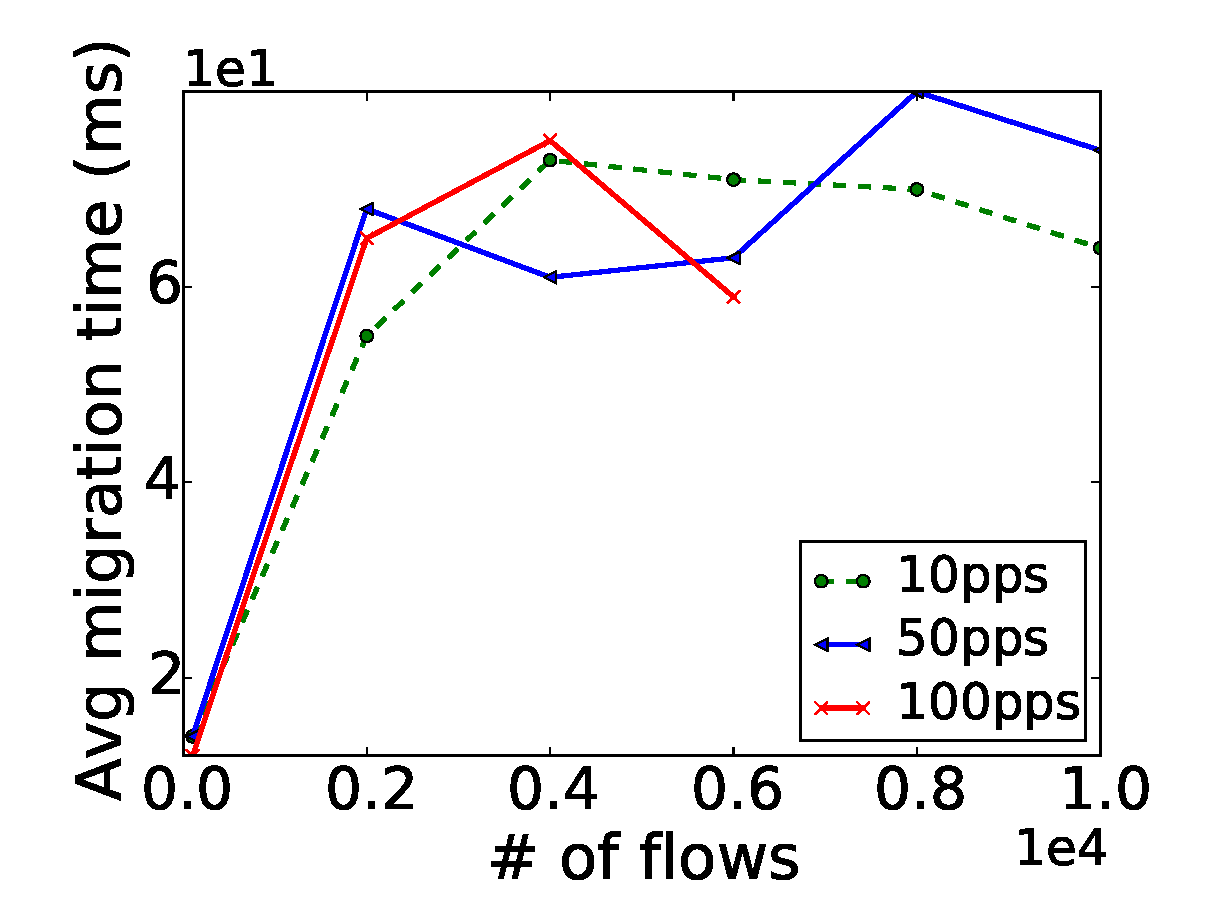
\includegraphics[width=\columnwidth]{figure/multi_flows_avg_migration_time.pdf}
		\caption{The average flow migration time of a single flow when migrating different number of flows.}\label{fig:avg-time-mig}
	 \end{subfigure}
\caption{The flow migration performance of \nfactor}
\label{fig:mig-perf}
\end{figure}

We present the evaluation result of flow migration in this section. In order to evaluate flow migration performance, we initialize the cluster with 2 runtimes running with 2 worker threads and then generate flows to one of the runtimes. Each flow is processed by the service chain consisting of all the 3 NF modules. We generate different number of flows, each flow has the same per-flow packet rate. In order to see how the evaluation performs under different per-flow packet rate, we also tune the per-flow packet rate with 10pps, 50pps and 100pps. When all the flows arrive on the migration source runtime. The migration source runtime starts migrating all the flows to the other runtime in the cluster. We calculate the total migration time and the average per-flow migration time. In order to control the workload during the migration, the runtime only allows 1000 concurrent migrations all the time. The result of this evaluation is shown in figure \ref{fig:mig-perf}.

We can see that as the number of migrated flows increase, the migration completion time increases almost linearly. This is because the average flow migration time remains almost a constant value and the runtime controls the maximum number of concurrent migrations. Note that when the system is not overloaded at all (100 flows), the average flow migration completion time is as small as 636us.  

When the per-flow packet rate is 100pps, the maximum number of flows that we use to evaluate the system is 6000. Continuing the evaluation with 8000 and 10000 flows just overloads the runtime as shown in figure \ref{fig:normal-performance}. 

 \begin{figure}[!t]
 \begin{subfigure}[t]{0.49\linewidth}
		\centering
		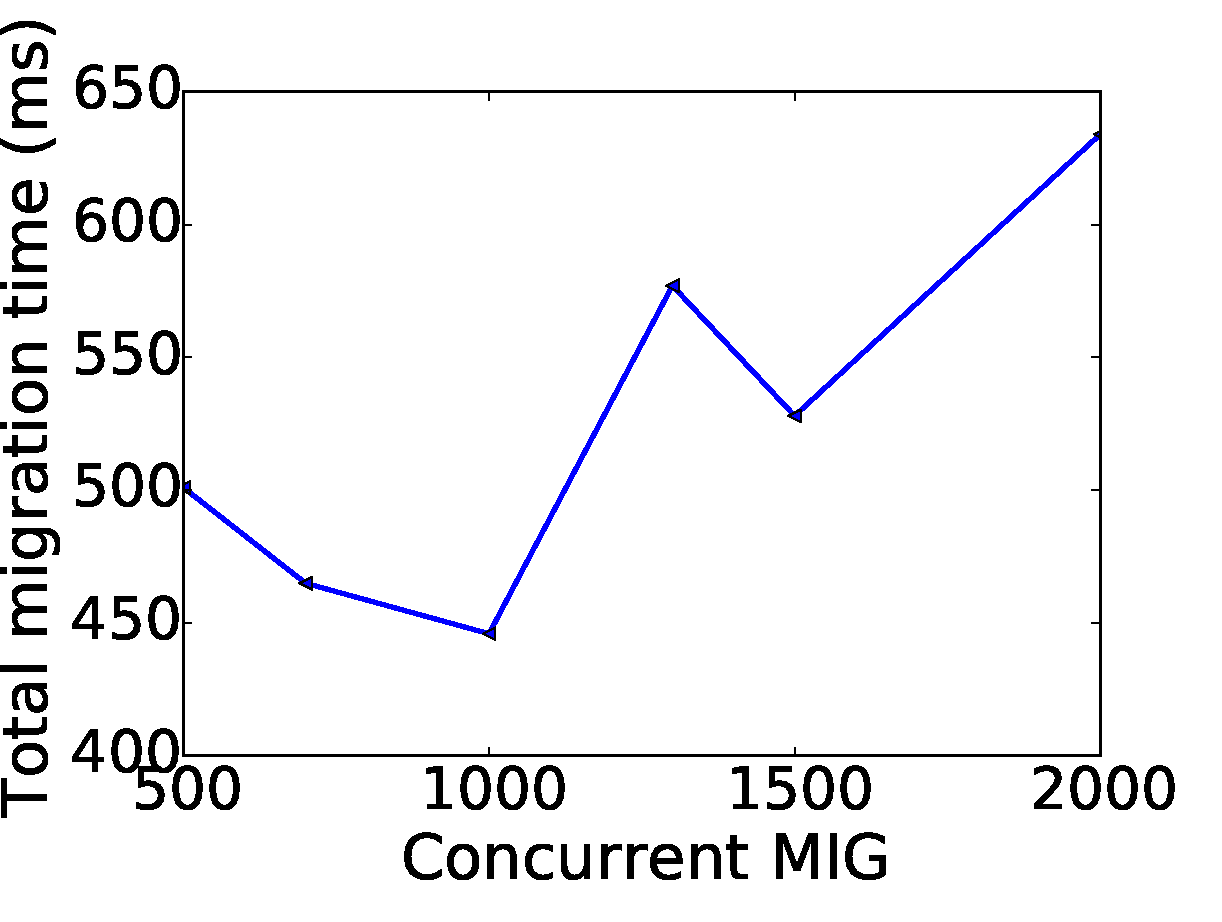
\includegraphics[width=\columnwidth]{figure/vary_batch_tot_migration_time.pdf}
		\caption{The total time to migrate all the flows when changing the maximum concurrent migrations.}\label{fig:avg-time-batch-mig}
	 \end{subfigure}\hfill
	 \begin{subfigure}[t]{0.49\linewidth}
	\centering
		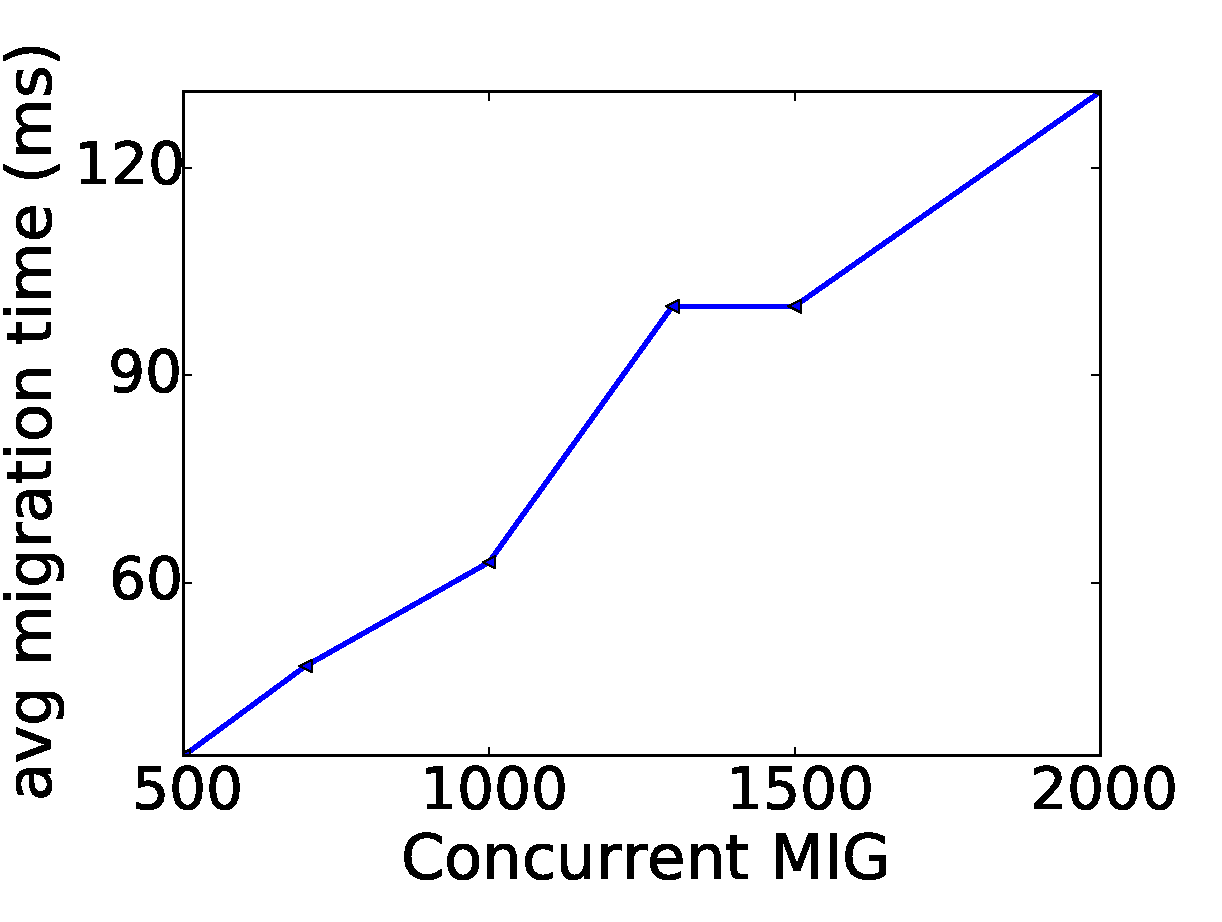
\includegraphics[width=\columnwidth]{figure/vary_batch_avg_migration_time.pdf}
		\caption{The average flow migration time of a single flow when changing the maximum concurrent migrations.}\label{fig:avg-mig-batch} \end{subfigure}
	\caption{The flow migration performance of \nfactor~when changing the maximum concurrent migrations.}
\label{fig:mig-perf}
\end{figure}

Since we control the number of concurrent migrations, we also want to see what happens if we change the number of concurrent migrations. We generate 6000 flows, each with 50 pps per-flow packet rate, and change the the number of concurrent migrations. The result of this evaluation is shown in fig \ref{fig:mig-perf}. As we can see from fig \ref{fig:avg-mig-batch}, increasing the maximum concurrent migrations increase the average flow migration completion time. However, whether the total flow migration completion time increased depends on the total number of flows that wait to be migrated. From the result of fig \ref{fig:avg-time-mig}, the choice of 1000 concurrent migrations sits in the sweat spot and accelerates the overall migration process.

 \begin{figure}[!t]
		\centering
		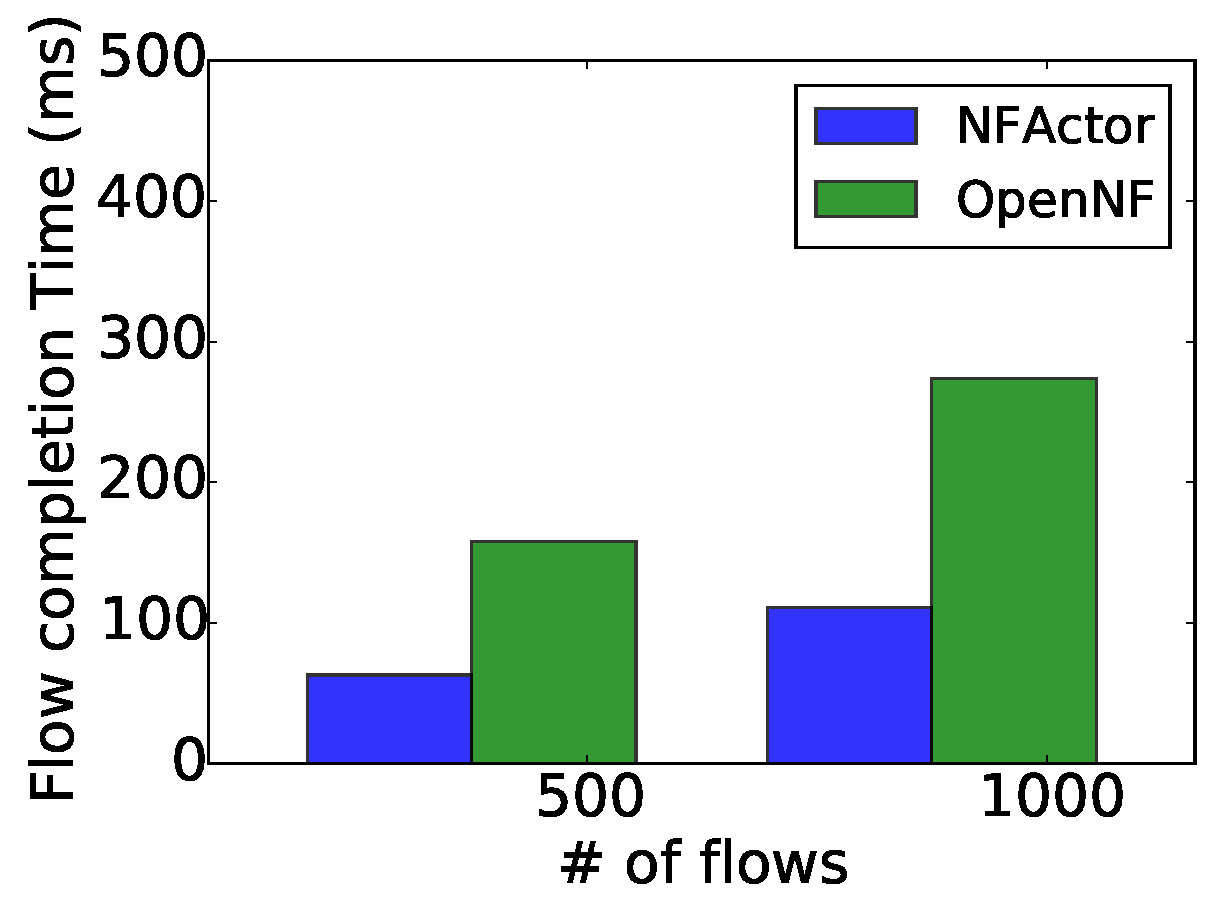
\includegraphics[width=0.6\columnwidth]{figure/opennf_nfactor_cmpFlowtime.pdf}
		\caption{The flow migration performance of \nfactor. Each flow in \nfactor~runtime goes through the service chain consisting of the 3 customzied NF modules. OpenNF controlls PRADS asset monitors.}
\label{fig:compare-opennf}
\end{figure}

Finally, we compare the flow migration performance of \nfactor~against OpenNF \cite{gember2015opennf}. We generate the same number of flows to both \nfactor~runtimes and NFs controlled by OpenNF and calculate the total time to migrate these flows. The evaluation result is shown in figure \ref{fig:compare-opennf}. Under both settings, the migration completion time of \nfactor~is more than 50\% faster than OpenNF.  This performance gain primarily comes from the simplified migration protocol design with the help of actor framework. In \nfactor, a flow migration process only involves transmitting 3 request-responses. Under light workload, the flow migration can complete within several hundreds of microseconds. Under high workload, \nfactor~runtime system controls the maximum number of concurrent migrations to control the migration workload, which may increase the migration performance as indicated in figure \ref{fig:avg-time-batch-mig}. All of these factors contribute to the improved flow migration performance of \nfactor~framework.

\subsection{Replication Performance}
\label{sec:rp}

 \begin{figure}[!t]
 \begin{subfigure}[t]{0.49\linewidth}
		\centering
		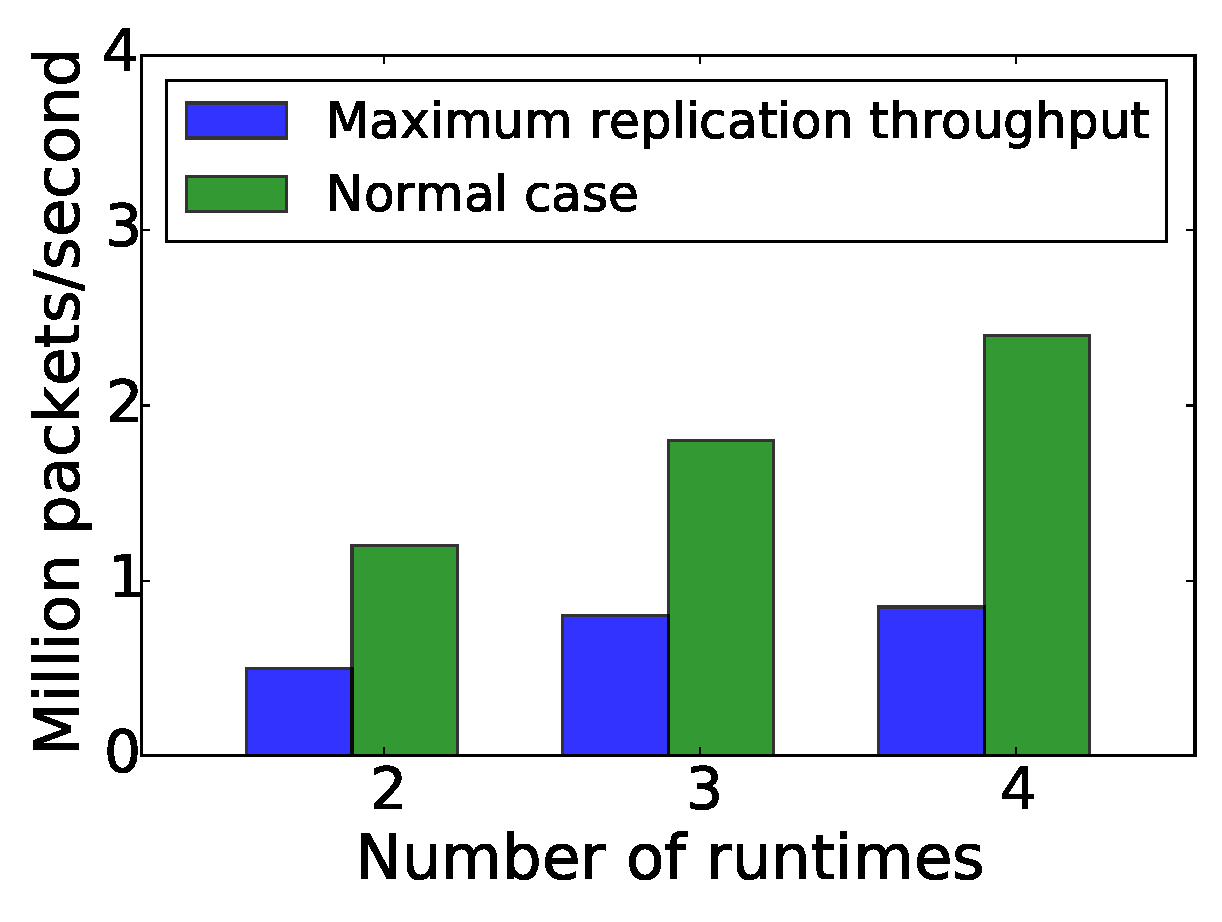
\includegraphics[width=\columnwidth]{figure/runtime_pktthroughput_cmp.pdf}
		\caption{The packet throughput of a \nfactor~cluster when replication is enabled. The throughput is compared against the throughput when replication is disabled. }\label{fig:rep-scale}
	 \end{subfigure}\hfill
	 \begin{subfigure}[t]{0.49\linewidth}
	\centering
		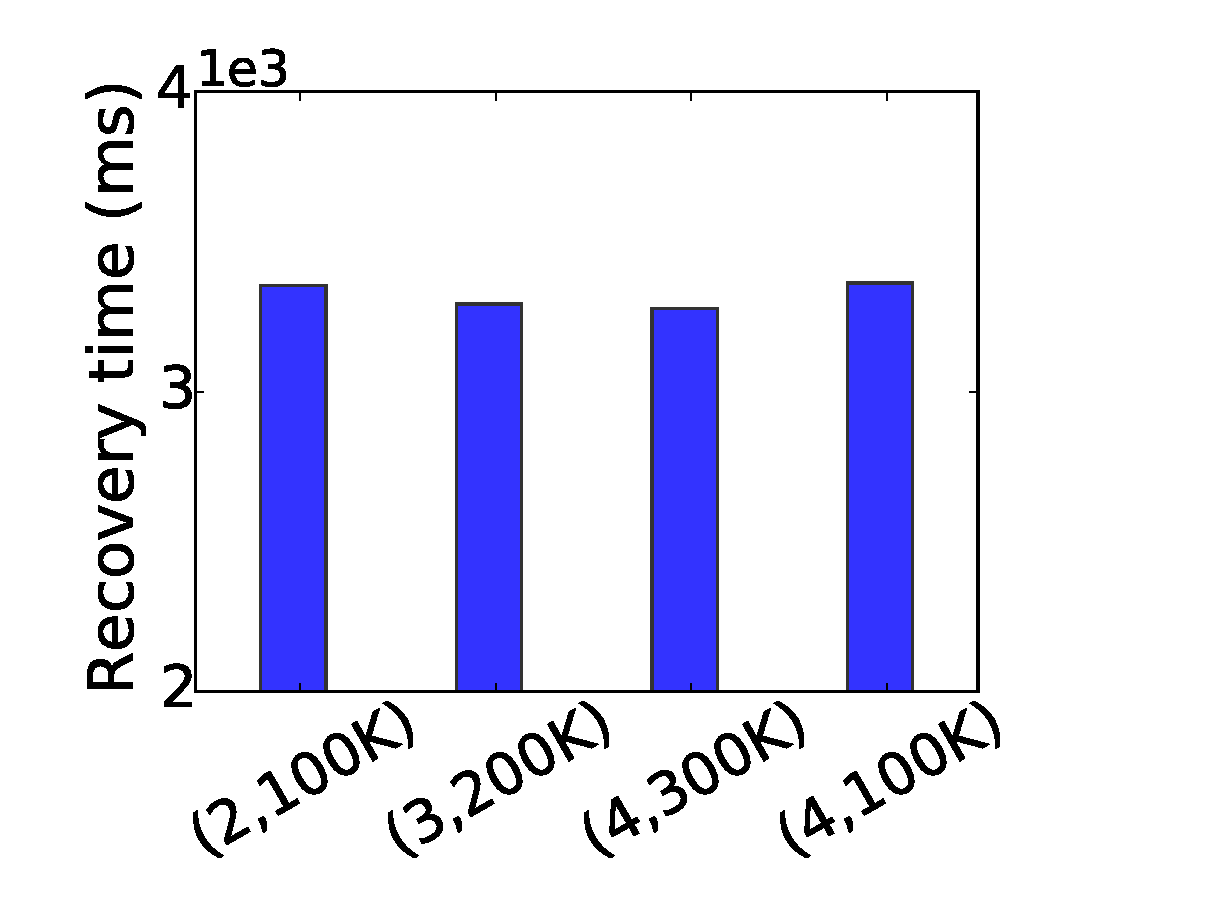
\includegraphics[width=\columnwidth]{figure/runtime_recovery_time.pdf}
		\caption{The recovery time of a failed runtime under different settings. The tuple on the $x$ axis represents the number of the runtime used in the evaluation and the total input packet rate. }\label{fig:rep-recovery} \end{subfigure}
	\caption{The flow migration performance of \nfactor}
\label{fig:rep-perf}
\end{figure}

In this section, we present the flow state replication evaluation result. In our evaluation, the actor creates a flow snapshot for every 10 flow packets that it has processed. Then it sends the flow state snapshot to the replica storage. In this evaluation, we first generate flows to the \nfactor~cluster to test the maximum throughput of a \nfactor~cluster when enabling replication. Then we calculate the recovery time of failed \nfactor~runtime. The recovery time is the from time that the controller detects a \nfactor~runtime failure, to the time that the recovered \nfactor~finishes replaying all of its replicas and responds to the controller to rejoin the cluster. Through out this evaluation, the runtime uses the service chain consisting of the 3 NF modules to process the flow. The result of the evaluation is shown in figure \ref{fig:rep-perf}. 

In figure \ref{fig:rep-scale}, we can see that there is an obvious overhead to enable replication on \nfactor~runtimes. The overall throughput when replication is enabled drops around 60\%. This is due to the large amount of replication messages that are exchanged during the replication process. Internally, the replication messages are sent over Linux kernel networking stack, which involves data copy and context switching, thus increasing the performance overhead of using replication. However, the overall throughput when replication is enabled could scale to 850K pps when 4 runtimes are used, which is enough to use in some restricted settings. 

Finally, figure \ref{fig:rep-recovery} shows the recovery time of \nfactor~runtime when replication is enabled. We found that the recovery time remains a consistent value of 3.3s, no matter how many runtimes are used or how large the input traffic is. The reason of this consistent recovery time is that the \nfactor~runtime maintains one replica on every other \nfactor~runtimes in the cluster. During recovery, several recovery threads are launched to fetch only one replica from another runtime. Then each recovery thread independently recovers actors by replaying its own replica. In this way, the recovery process is fully distributed and scales well as the number of replica increases. Note is that the average time it takes for a recovered runtime to fetch all the replicas and recover all of its actors is only 1.2s. So actually around 2.1s is spent in container creation and connection establishment. 

%\section{Discussion}
\label{sec:discussion}

Discuss the limitations of NFActor here.
\section{Related Work}
\label{sec:relatedwork}

%Discuss related work here.

%\chuan{remember to discuss the EuroSys’16 work ``Optimizing Distributed Actor Systems for Dynamic Interactive Services''}


\textbf{Network Function Virtualization (NFV).} NFV is a new trend that advocates moving from running hardware middleboxes to running software network function instances in virtualized environment. The literature has developed a broad range of NFV applications, from scaling and controlling the NFV systems \cite{gember2012stratos, palkar2015e2}, to improving the performance of NFV software \cite{hwang2015netvm, Han:EECS-2015-155, martins2014clickos, 199352}, to migrating flows among different NF instances \cite{rajagopalan2013split, khalid2016paving, gember2015opennf}, and to replicating NF instances \cite{rajagopalan2013pico, sherry2015rollback}. However, none of the above mentioned systems provide a uniform runtime platform to execute network functions. Most of the NF instances are still created as a standalone software running inside virtual machine or containers. Even though modular design introduced by ClickOS \cite{kohler2000click} simplifies the way of how NF functions are constructed, however, nowadays there are new demands for NFV system, which require advanced control functionality to be integrated even into the NF softwares. 

Among the advanced control functionality, flow migration and fault tolerance are definitely the two of the most important features. Existing work such as OpenNF \cite{gember2015opennf} and Split/Merge \cite{rajagopalan2013split} requires direct modification to the core processing logic of NF softwares, which is tedious and hard to do. On the other hand, existing work rely on SDN to carry out migration protocol, thereby increasing the complexity of the migration protocol. Finally, the migration process is fully controlled by a  centralized SDN controller, which may not be scalable if there are many NF instances that need flow migration service. The proposed NFActor framework overcomes most of the above mentioned obstacles by providing a uniform runtime system constructed with actor framework. The actors could be migrated by themselves without the coordination from a centralized controller. The framework provides a  fast virtual switch to substitute the functionality of a dedicated SDN switch. With the help of the actor framework and the customized virtual switch, the migration protocol only needs to transmit 3 request-responses. Finally, the NFActor achieves transparent migration without the need for manual modification of the NF software. This greatly simplifies the the required procedures for using migration service.

Another important control functionality lies on replication. The replication process usually involves check-pointing the entire process image and making a back-up for the created process image \cite{sherry2015rollback}, which may halt the execution of the NF software, leading to packet losses. NFActor framework is able to check-point of the state of the flow, which is relatively lightweight to do and does not incur a high latency overhead. Similar with migration process, NF modules written using NFActor framework could be transparently replicated. Existing work like \cite{sherry2015rollback} rely on automated tools to extract important state variables for replicating.

\textbf{Actor Programming Model.} The actor programming model has been widely used to construct resilient distributed software \cite{erlang, akka, Orleans, caf}. The actors are asynchronous entities that can receive and send messages as if they are running in a dedicated process. The actors usually run on a powerful runtime system \cite{erlang, akka, caf}, enabling them to achieve network transparency. It greatly simplifies programming with actor model. Even though actor programming model is widely used in both the industry and academic worlds, we have not found any related work that leverage actor programming model to construct NFV system, even though there is a natural connection among actor message processing and NF flow processing. Reliazing this problem, we are the first one to introduce actor programming model into NFV system and shows that using actor programming model can really bring benefits for designing NFV applications.

\textbf{Lightweight Execution Context. } There has been a study on constructing lightweight execution context \cite{litton2016light} in kernel. In this work, the authors construct a light weight execution context by creating multiple memory mapping table in the same process. Switching among different memory tables could be viewed as switching among different lightweight execution contexts. NFActor provides a similar execution context, not for kernel processes, but for network functions. Each actor inside NFActor framework actually provides a lightweight execution context for processing a packet along a service chain. Being a lightweight context, the actors do not introduce too much overhead as we can see from the experiment session. On the other hand, packet processing is fully monitored by the execution context, thereby providing a transparent way to migrate and replicate flow states.









\section{Conclusion}
\label{sec:conclusion}

In this work, we present a new framework for building resilient NFV system, called NFActor framework. Unlike existing NFV system, where NF instances run as a program inside a virtual machine or a container, NFActor framework provides a set of API to implement NF modules which executes on the runtime system of NFActor framework. Inside the NFActor framework, packet processing of a flow is dedicated to an actor. The actor provides an execution context for processing packets along the service chain, reacting to flow migration and replication messages. NF modules written using the API provided by NFActor framework achieves flow migration and state replication functionalities in a transparent fashion. The implementer of the NF module therefore only needs to concentrate on designing the core logic. Evaluation result shows that even though the NFActor framework incurs some overhead when processing packets, the scalability of NFActor runtime is good enough to support line-speed requirement. NFActor framework outperforms existing works by more than 50\% in flow migration completion time. Finally, the flow state replication of NFActor is scalable and achieves consistent recovery time.

\bibliographystyle{abbrv}
\bibliography{bibliography}

\end{document}
